\DeclareUnicodeCharacter{041B}{\CYRL}



\documentclass[11pt]{article}

    
    
    \usepackage[breakable]{tcolorbox}
    \usepackage{parskip} % Stop auto-indenting (to mimic markdown behaviour)
    \usepackage[english,russian]{babel}
    \usepackage{graphicx}
    \usepackage{subcaption}
    

    % Basic figure setup, for now with no caption control since it's done
    % automatically by Pandoc (which extracts ![](path) syntax from Markdown).
    \usepackage{graphicx}
    % Maintain compatibility with old templates. Remove in nbconvert 6.0
    \let\Oldincludegraphics\includegraphics
    % Ensure that by default, figures have no caption (until we provide a
    % proper Figure object with a Caption API and a way to capture that
    % in the conversion process - todo).
    \usepackage{caption}
    \DeclareCaptionFormat{nocaption}{}
    \captionsetup{format=nocaption,aboveskip=0pt,belowskip=0pt}

    \usepackage{float}
    \floatplacement{figure}{H} % forces figures to be placed at the correct location
    \usepackage{xcolor} % Allow colors to be defined
    \usepackage{enumerate} % Needed for markdown enumerations to work
    \usepackage{geometry} % Used to adjust the document margins
    \usepackage{amsmath} % Equations
    \usepackage{amssymb} % Equations
    \usepackage{textcomp} % defines textquotesingle
    % Hack from http://tex.stackexchange.com/a/47451/13684:
    \AtBeginDocument{%
        \def\PYZsq{\textquotesingle}% Upright quotes in Pygmentized code
    }
    \usepackage{upquote} % Upright quotes for verbatim code
    \usepackage{eurosym} % defines \euro

    \usepackage{iftex}
    \ifPDFTeX
        \usepackage[T1]{fontenc}
        \IfFileExists{alphabeta.sty}{
              \usepackage{alphabeta}
          }{
              \usepackage[mathletters]{ucs}
              \usepackage[utf8x]{inputenc}
          }
    \else
        \usepackage{fontspec}
        \usepackage{unicode-math}
    \fi

    \usepackage{fancyvrb} % verbatim replacement that allows latex
    \usepackage{grffile} % extends the file name processing of package graphics
                         % to support a larger range
    \makeatletter % fix for old versions of grffile with XeLaTeX
    \@ifpackagelater{grffile}{2019/11/01}
    {
      % Do nothing on new versions
    }
    {
      \def\Gread@@xetex#1{%
        \IfFileExists{"\Gin@base".bb}%
        {\Gread@eps{\Gin@base.bb}}%
        {\Gread@@xetex@aux#1}%
      }
    }
    \makeatother
    \usepackage[Export]{adjustbox} % Used to constrain images to a maximum size
    \adjustboxset{max size={0.9\linewidth}{0.9\paperheight}}

    % The hyperref package gives us a pdf with properly built
    % internal navigation ('pdf bookmarks' for the table of contents,
    % internal cross-reference links, web links for URLs, etc.)
    \usepackage{hyperref}
    % The default LaTeX title has an obnoxious amount of whitespace. By default,
    % titling removes some of it. It also provides customization options.
    \usepackage{titling}
    \usepackage{longtable} % longtable support required by pandoc >1.10
    \usepackage{booktabs}  % table support for pandoc > 1.12.2
    \usepackage{array}     % table support for pandoc >= 2.11.3
    \usepackage{calc}      % table minipage width calculation for pandoc >= 2.11.1
    \usepackage[inline]{enumitem} % IRkernel/repr support (it uses the enumerate* environment)
    \usepackage[normalem]{ulem} % ulem is needed to support strikethroughs (\sout)
                                % normalem makes italics be italics, not underlines
    \usepackage{mathrsfs}
    

    
    % Colors for the hyperref package
    \definecolor{urlcolor}{rgb}{0,.145,.698}
    \definecolor{linkcolor}{rgb}{.71,0.21,0.01}
    \definecolor{citecolor}{rgb}{.12,.54,.11}

    % ANSI colors
    \definecolor{ansi-black}{HTML}{3E424D}
    \definecolor{ansi-black-intense}{HTML}{282C36}
    \definecolor{ansi-red}{HTML}{E75C58}
    \definecolor{ansi-red-intense}{HTML}{B22B31}
    \definecolor{ansi-green}{HTML}{00A250}
    \definecolor{ansi-green-intense}{HTML}{007427}
    \definecolor{ansi-yellow}{HTML}{DDB62B}
    \definecolor{ansi-yellow-intense}{HTML}{B27D12}
    \definecolor{ansi-blue}{HTML}{208FFB}
    \definecolor{ansi-blue-intense}{HTML}{0065CA}
    \definecolor{ansi-magenta}{HTML}{D160C4}
    \definecolor{ansi-magenta-intense}{HTML}{A03196}
    \definecolor{ansi-cyan}{HTML}{60C6C8}
    \definecolor{ansi-cyan-intense}{HTML}{258F8F}
    \definecolor{ansi-white}{HTML}{C5C1B4}
    \definecolor{ansi-white-intense}{HTML}{A1A6B2}
    \definecolor{ansi-default-inverse-fg}{HTML}{FFFFFF}
    \definecolor{ansi-default-inverse-bg}{HTML}{000000}

    % common color for the border for error outputs.
    \definecolor{outerrorbackground}{HTML}{FFDFDF}

    % commands and environments needed by pandoc snippets
    % extracted from the output of `pandoc -s`
    \providecommand{\tightlist}{%
      \setlength{\itemsep}{0pt}\setlength{\parskip}{0pt}}
    \DefineVerbatimEnvironment{Highlighting}{Verbatim}{commandchars=\\\{\}}
    % Add ',fontsize=\small' for more characters per line
    \newenvironment{Shaded}{}{}
    \newcommand{\KeywordTok}[1]{\textcolor[rgb]{0.00,0.44,0.13}{\textbf{{#1}}}}
    \newcommand{\DataTypeTok}[1]{\textcolor[rgb]{0.56,0.13,0.00}{{#1}}}
    \newcommand{\DecValTok}[1]{\textcolor[rgb]{0.25,0.63,0.44}{{#1}}}
    \newcommand{\BaseNTok}[1]{\textcolor[rgb]{0.25,0.63,0.44}{{#1}}}
    \newcommand{\FloatTok}[1]{\textcolor[rgb]{0.25,0.63,0.44}{{#1}}}
    \newcommand{\CharTok}[1]{\textcolor[rgb]{0.25,0.44,0.63}{{#1}}}
    \newcommand{\StringTok}[1]{\textcolor[rgb]{0.25,0.44,0.63}{{#1}}}
    \newcommand{\CommentTok}[1]{\textcolor[rgb]{0.38,0.63,0.69}{\textit{{#1}}}}
    \newcommand{\OtherTok}[1]{\textcolor[rgb]{0.00,0.44,0.13}{{#1}}}
    \newcommand{\AlertTok}[1]{\textcolor[rgb]{1.00,0.00,0.00}{\textbf{{#1}}}}
    \newcommand{\FunctionTok}[1]{\textcolor[rgb]{0.02,0.16,0.49}{{#1}}}
    \newcommand{\RegionMarkerTok}[1]{{#1}}
    \newcommand{\ErrorTok}[1]{\textcolor[rgb]{1.00,0.00,0.00}{\textbf{{#1}}}}
    \newcommand{\NormalTok}[1]{{#1}}

    % Additional commands for more recent versions of Pandoc
    \newcommand{\ConstantTok}[1]{\textcolor[rgb]{0.53,0.00,0.00}{{#1}}}
    \newcommand{\SpecialCharTok}[1]{\textcolor[rgb]{0.25,0.44,0.63}{{#1}}}
    \newcommand{\VerbatimStringTok}[1]{\textcolor[rgb]{0.25,0.44,0.63}{{#1}}}
    \newcommand{\SpecialStringTok}[1]{\textcolor[rgb]{0.73,0.40,0.53}{{#1}}}
    \newcommand{\ImportTok}[1]{{#1}}
    \newcommand{\DocumentationTok}[1]{\textcolor[rgb]{0.73,0.13,0.13}{\textit{{#1}}}}
    \newcommand{\AnnotationTok}[1]{\textcolor[rgb]{0.38,0.63,0.69}{\textbf{\textit{{#1}}}}}
    \newcommand{\CommentVarTok}[1]{\textcolor[rgb]{0.38,0.63,0.69}{\textbf{\textit{{#1}}}}}
    \newcommand{\VariableTok}[1]{\textcolor[rgb]{0.10,0.09,0.49}{{#1}}}
    \newcommand{\ControlFlowTok}[1]{\textcolor[rgb]{0.00,0.44,0.13}{\textbf{{#1}}}}
    \newcommand{\OperatorTok}[1]{\textcolor[rgb]{0.40,0.40,0.40}{{#1}}}
    \newcommand{\BuiltInTok}[1]{{#1}}
    \newcommand{\ExtensionTok}[1]{{#1}}
    \newcommand{\PreprocessorTok}[1]{\textcolor[rgb]{0.74,0.48,0.00}{{#1}}}
    \newcommand{\AttributeTok}[1]{\textcolor[rgb]{0.49,0.56,0.16}{{#1}}}
    \newcommand{\InformationTok}[1]{\textcolor[rgb]{0.38,0.63,0.69}{\textbf{\textit{{#1}}}}}
    \newcommand{\WarningTok}[1]{\textcolor[rgb]{0.38,0.63,0.69}{\textbf{\textit{{#1}}}}}


    % Define a nice break command that doesn't care if a line doesn't already
    % exist.
    \def\br{\hspace*{\fill} \\* }
    % Math Jax compatibility definitions
    \def\gt{>}
    \def\lt{<}
    \let\Oldtex\TeX
    \let\Oldlatex\LaTeX
    \renewcommand{\TeX}{\textrm{\Oldtex}}
    \renewcommand{\LaTeX}{\textrm{\Oldlatex}}
    % Document parameters
    % Document title
    \title{CHM\_Lab1}
    
    
    
    
    
% Pygments definitions
\makeatletter
\def\PY@reset{\let\PY@it=\relax \let\PY@bf=\relax%
    \let\PY@ul=\relax \let\PY@tc=\relax%
    \let\PY@bc=\relax \let\PY@ff=\relax}
\def\PY@tok#1{\csname PY@tok@#1\endcsname}
\def\PY@toks#1+{\ifx\relax#1\empty\else%
    \PY@tok{#1}\expandafter\PY@toks\fi}
\def\PY@do#1{\PY@bc{\PY@tc{\PY@ul{%
    \PY@it{\PY@bf{\PY@ff{#1}}}}}}}
\def\PY#1#2{\PY@reset\PY@toks#1+\relax+\PY@do{#2}}

\@namedef{PY@tok@w}{\def\PY@tc##1{\textcolor[rgb]{0.73,0.73,0.73}{##1}}}
\@namedef{PY@tok@c}{\let\PY@it=\textit\def\PY@tc##1{\textcolor[rgb]{0.24,0.48,0.48}{##1}}}
\@namedef{PY@tok@cp}{\def\PY@tc##1{\textcolor[rgb]{0.61,0.40,0.00}{##1}}}
\@namedef{PY@tok@k}{\let\PY@bf=\textbf\def\PY@tc##1{\textcolor[rgb]{0.00,0.50,0.00}{##1}}}
\@namedef{PY@tok@kp}{\def\PY@tc##1{\textcolor[rgb]{0.00,0.50,0.00}{##1}}}
\@namedef{PY@tok@kt}{\def\PY@tc##1{\textcolor[rgb]{0.69,0.00,0.25}{##1}}}
\@namedef{PY@tok@o}{\def\PY@tc##1{\textcolor[rgb]{0.40,0.40,0.40}{##1}}}
\@namedef{PY@tok@ow}{\let\PY@bf=\textbf\def\PY@tc##1{\textcolor[rgb]{0.67,0.13,1.00}{##1}}}
\@namedef{PY@tok@nb}{\def\PY@tc##1{\textcolor[rgb]{0.00,0.50,0.00}{##1}}}
\@namedef{PY@tok@nf}{\def\PY@tc##1{\textcolor[rgb]{0.00,0.00,1.00}{##1}}}
\@namedef{PY@tok@nc}{\let\PY@bf=\textbf\def\PY@tc##1{\textcolor[rgb]{0.00,0.00,1.00}{##1}}}
\@namedef{PY@tok@nn}{\let\PY@bf=\textbf\def\PY@tc##1{\textcolor[rgb]{0.00,0.00,1.00}{##1}}}
\@namedef{PY@tok@ne}{\let\PY@bf=\textbf\def\PY@tc##1{\textcolor[rgb]{0.80,0.25,0.22}{##1}}}
\@namedef{PY@tok@nv}{\def\PY@tc##1{\textcolor[rgb]{0.10,0.09,0.49}{##1}}}
\@namedef{PY@tok@no}{\def\PY@tc##1{\textcolor[rgb]{0.53,0.00,0.00}{##1}}}
\@namedef{PY@tok@nl}{\def\PY@tc##1{\textcolor[rgb]{0.46,0.46,0.00}{##1}}}
\@namedef{PY@tok@ni}{\let\PY@bf=\textbf\def\PY@tc##1{\textcolor[rgb]{0.44,0.44,0.44}{##1}}}
\@namedef{PY@tok@na}{\def\PY@tc##1{\textcolor[rgb]{0.41,0.47,0.13}{##1}}}
\@namedef{PY@tok@nt}{\let\PY@bf=\textbf\def\PY@tc##1{\textcolor[rgb]{0.00,0.50,0.00}{##1}}}
\@namedef{PY@tok@nd}{\def\PY@tc##1{\textcolor[rgb]{0.67,0.13,1.00}{##1}}}
\@namedef{PY@tok@s}{\def\PY@tc##1{\textcolor[rgb]{0.73,0.13,0.13}{##1}}}
\@namedef{PY@tok@sd}{\let\PY@it=\textit\def\PY@tc##1{\textcolor[rgb]{0.73,0.13,0.13}{##1}}}
\@namedef{PY@tok@si}{\let\PY@bf=\textbf\def\PY@tc##1{\textcolor[rgb]{0.64,0.35,0.47}{##1}}}
\@namedef{PY@tok@se}{\let\PY@bf=\textbf\def\PY@tc##1{\textcolor[rgb]{0.67,0.36,0.12}{##1}}}
\@namedef{PY@tok@sr}{\def\PY@tc##1{\textcolor[rgb]{0.64,0.35,0.47}{##1}}}
\@namedef{PY@tok@ss}{\def\PY@tc##1{\textcolor[rgb]{0.10,0.09,0.49}{##1}}}
\@namedef{PY@tok@sx}{\def\PY@tc##1{\textcolor[rgb]{0.00,0.50,0.00}{##1}}}
\@namedef{PY@tok@m}{\def\PY@tc##1{\textcolor[rgb]{0.40,0.40,0.40}{##1}}}
\@namedef{PY@tok@gh}{\let\PY@bf=\textbf\def\PY@tc##1{\textcolor[rgb]{0.00,0.00,0.50}{##1}}}
\@namedef{PY@tok@gu}{\let\PY@bf=\textbf\def\PY@tc##1{\textcolor[rgb]{0.50,0.00,0.50}{##1}}}
\@namedef{PY@tok@gd}{\def\PY@tc##1{\textcolor[rgb]{0.63,0.00,0.00}{##1}}}
\@namedef{PY@tok@gi}{\def\PY@tc##1{\textcolor[rgb]{0.00,0.52,0.00}{##1}}}
\@namedef{PY@tok@gr}{\def\PY@tc##1{\textcolor[rgb]{0.89,0.00,0.00}{##1}}}
\@namedef{PY@tok@ge}{\let\PY@it=\textit}
\@namedef{PY@tok@gs}{\let\PY@bf=\textbf}
\@namedef{PY@tok@gp}{\let\PY@bf=\textbf\def\PY@tc##1{\textcolor[rgb]{0.00,0.00,0.50}{##1}}}
\@namedef{PY@tok@go}{\def\PY@tc##1{\textcolor[rgb]{0.44,0.44,0.44}{##1}}}
\@namedef{PY@tok@gt}{\def\PY@tc##1{\textcolor[rgb]{0.00,0.27,0.87}{##1}}}
\@namedef{PY@tok@err}{\def\PY@bc##1{{\setlength{\fboxsep}{\string -\fboxrule}\fcolorbox[rgb]{1.00,0.00,0.00}{1,1,1}{\strut ##1}}}}
\@namedef{PY@tok@kc}{\let\PY@bf=\textbf\def\PY@tc##1{\textcolor[rgb]{0.00,0.50,0.00}{##1}}}
\@namedef{PY@tok@kd}{\let\PY@bf=\textbf\def\PY@tc##1{\textcolor[rgb]{0.00,0.50,0.00}{##1}}}
\@namedef{PY@tok@kn}{\let\PY@bf=\textbf\def\PY@tc##1{\textcolor[rgb]{0.00,0.50,0.00}{##1}}}
\@namedef{PY@tok@kr}{\let\PY@bf=\textbf\def\PY@tc##1{\textcolor[rgb]{0.00,0.50,0.00}{##1}}}
\@namedef{PY@tok@bp}{\def\PY@tc##1{\textcolor[rgb]{0.00,0.50,0.00}{##1}}}
\@namedef{PY@tok@fm}{\def\PY@tc##1{\textcolor[rgb]{0.00,0.00,1.00}{##1}}}
\@namedef{PY@tok@vc}{\def\PY@tc##1{\textcolor[rgb]{0.10,0.09,0.49}{##1}}}
\@namedef{PY@tok@vg}{\def\PY@tc##1{\textcolor[rgb]{0.10,0.09,0.49}{##1}}}
\@namedef{PY@tok@vi}{\def\PY@tc##1{\textcolor[rgb]{0.10,0.09,0.49}{##1}}}
\@namedef{PY@tok@vm}{\def\PY@tc##1{\textcolor[rgb]{0.10,0.09,0.49}{##1}}}
\@namedef{PY@tok@sa}{\def\PY@tc##1{\textcolor[rgb]{0.73,0.13,0.13}{##1}}}
\@namedef{PY@tok@sb}{\def\PY@tc##1{\textcolor[rgb]{0.73,0.13,0.13}{##1}}}
\@namedef{PY@tok@sc}{\def\PY@tc##1{\textcolor[rgb]{0.73,0.13,0.13}{##1}}}
\@namedef{PY@tok@dl}{\def\PY@tc##1{\textcolor[rgb]{0.73,0.13,0.13}{##1}}}
\@namedef{PY@tok@s2}{\def\PY@tc##1{\textcolor[rgb]{0.73,0.13,0.13}{##1}}}
\@namedef{PY@tok@sh}{\def\PY@tc##1{\textcolor[rgb]{0.73,0.13,0.13}{##1}}}
\@namedef{PY@tok@s1}{\def\PY@tc##1{\textcolor[rgb]{0.73,0.13,0.13}{##1}}}
\@namedef{PY@tok@mb}{\def\PY@tc##1{\textcolor[rgb]{0.40,0.40,0.40}{##1}}}
\@namedef{PY@tok@mf}{\def\PY@tc##1{\textcolor[rgb]{0.40,0.40,0.40}{##1}}}
\@namedef{PY@tok@mh}{\def\PY@tc##1{\textcolor[rgb]{0.40,0.40,0.40}{##1}}}
\@namedef{PY@tok@mi}{\def\PY@tc##1{\textcolor[rgb]{0.40,0.40,0.40}{##1}}}
\@namedef{PY@tok@il}{\def\PY@tc##1{\textcolor[rgb]{0.40,0.40,0.40}{##1}}}
\@namedef{PY@tok@mo}{\def\PY@tc##1{\textcolor[rgb]{0.40,0.40,0.40}{##1}}}
\@namedef{PY@tok@ch}{\let\PY@it=\textit\def\PY@tc##1{\textcolor[rgb]{0.24,0.48,0.48}{##1}}}
\@namedef{PY@tok@cm}{\let\PY@it=\textit\def\PY@tc##1{\textcolor[rgb]{0.24,0.48,0.48}{##1}}}
\@namedef{PY@tok@cpf}{\let\PY@it=\textit\def\PY@tc##1{\textcolor[rgb]{0.24,0.48,0.48}{##1}}}
\@namedef{PY@tok@c1}{\let\PY@it=\textit\def\PY@tc##1{\textcolor[rgb]{0.24,0.48,0.48}{##1}}}
\@namedef{PY@tok@cs}{\let\PY@it=\textit\def\PY@tc##1{\textcolor[rgb]{0.24,0.48,0.48}{##1}}}

\def\PYZbs{\char`\\}
\def\PYZus{\char`\_}
\def\PYZob{\char`\{}
\def\PYZcb{\char`\}}
\def\PYZca{\char`\^}
\def\PYZam{\char`\&}
\def\PYZlt{\char`\<}
\def\PYZgt{\char`\>}
\def\PYZsh{\char`\#}
\def\PYZpc{\char`\%}
\def\PYZdl{\char`\$}
\def\PYZhy{\char`\-}
\def\PYZsq{\char`\'}
\def\PYZdq{\char`\"}
\def\PYZti{\char`\~}
% for compatibility with earlier versions
\def\PYZat{@}
\def\PYZlb{[}
\def\PYZrb{]}
\makeatother


    % For linebreaks inside Verbatim environment from package fancyvrb.
    \makeatletter
        \newbox\Wrappedcontinuationbox
        \newbox\Wrappedvisiblespacebox
        \newcommand*\Wrappedvisiblespace {\textcolor{red}{\textvisiblespace}}
        \newcommand*\Wrappedcontinuationsymbol {\textcolor{red}{\llap{\tiny$\m@th\hookrightarrow$}}}
        \newcommand*\Wrappedcontinuationindent {3ex }
        \newcommand*\Wrappedafterbreak {\kern\Wrappedcontinuationindent\copy\Wrappedcontinuationbox}
        % Take advantage of the already applied Pygments mark-up to insert
        % potential linebreaks for TeX processing.
        %        {, <, #, %, $, ' and ": go to next line.
        %        _, }, ^, &, >, - and ~: stay at end of broken line.
        % Use of \textquotesingle for straight quote.
        \newcommand*\Wrappedbreaksatspecials {%
            \def\PYGZus{\discretionary{\char`\_}{\Wrappedafterbreak}{\char`\_}}%
            \def\PYGZob{\discretionary{}{\Wrappedafterbreak\char`\{}{\char`\{}}%
            \def\PYGZcb{\discretionary{\char`\}}{\Wrappedafterbreak}{\char`\}}}%
            \def\PYGZca{\discretionary{\char`\^}{\Wrappedafterbreak}{\char`\^}}%
            \def\PYGZam{\discretionary{\char`\&}{\Wrappedafterbreak}{\char`\&}}%
            \def\PYGZlt{\discretionary{}{\Wrappedafterbreak\char`\<}{\char`\<}}%
            \def\PYGZgt{\discretionary{\char`\>}{\Wrappedafterbreak}{\char`\>}}%
            \def\PYGZsh{\discretionary{}{\Wrappedafterbreak\char`\#}{\char`\#}}%
            \def\PYGZpc{\discretionary{}{\Wrappedafterbreak\char`\%}{\char`\%}}%
            \def\PYGZdl{\discretionary{}{\Wrappedafterbreak\char`\$}{\char`\$}}%
            \def\PYGZhy{\discretionary{\char`\-}{\Wrappedafterbreak}{\char`\-}}%
            \def\PYGZsq{\discretionary{}{\Wrappedafterbreak\textquotesingle}{\textquotesingle}}%
            \def\PYGZdq{\discretionary{}{\Wrappedafterbreak\char`\"}{\char`\"}}%
            \def\PYGZti{\discretionary{\char`\~}{\Wrappedafterbreak}{\char`\~}}%
        }
        % Some characters . , ; ? ! / are not pygmentized.
        % This macro makes them "active" and they will insert potential linebreaks
        \newcommand*\Wrappedbreaksatpunct {%
            \lccode`\~`\.\lowercase{\def~}{\discretionary{\hbox{\char`\.}}{\Wrappedafterbreak}{\hbox{\char`\.}}}%
            \lccode`\~`\,\lowercase{\def~}{\discretionary{\hbox{\char`\,}}{\Wrappedafterbreak}{\hbox{\char`\,}}}%
            \lccode`\~`\;\lowercase{\def~}{\discretionary{\hbox{\char`\;}}{\Wrappedafterbreak}{\hbox{\char`\;}}}%
            \lccode`\~`\:\lowercase{\def~}{\discretionary{\hbox{\char`\:}}{\Wrappedafterbreak}{\hbox{\char`\:}}}%
            \lccode`\~`\?\lowercase{\def~}{\discretionary{\hbox{\char`\?}}{\Wrappedafterbreak}{\hbox{\char`\?}}}%
            \lccode`\~`\!\lowercase{\def~}{\discretionary{\hbox{\char`\!}}{\Wrappedafterbreak}{\hbox{\char`\!}}}%
            \lccode`\~`\/\lowercase{\def~}{\discretionary{\hbox{\char`\/}}{\Wrappedafterbreak}{\hbox{\char`\/}}}%
            \catcode`\.\active
            \catcode`\,\active
            \catcode`\;\active
            \catcode`\:\active
            \catcode`\?\active
            \catcode`\!\active
            \catcode`\/\active
            \lccode`\~`\~
        }
    \makeatother

    \let\OriginalVerbatim=\Verbatim
    \makeatletter
    \renewcommand{\Verbatim}[1][1]{%
        %\parskip\z@skip
        \sbox\Wrappedcontinuationbox {\Wrappedcontinuationsymbol}%
        \sbox\Wrappedvisiblespacebox {\FV@SetupFont\Wrappedvisiblespace}%
        \def\FancyVerbFormatLine ##1{\hsize\linewidth
            \vtop{\raggedright\hyphenpenalty\z@\exhyphenpenalty\z@
                \doublehyphendemerits\z@\finalhyphendemerits\z@
                \strut ##1\strut}%
        }%
        % If the linebreak is at a space, the latter will be displayed as visible
        % space at end of first line, and a continuation symbol starts next line.
        % Stretch/shrink are however usually zero for typewriter font.
        \def\FV@Space {%
            \nobreak\hskip\z@ plus\fontdimen3\font minus\fontdimen4\font
            \discretionary{\copy\Wrappedvisiblespacebox}{\Wrappedafterbreak}
            {\kern\fontdimen2\font}%
        }%

        % Allow breaks at special characters using \PYG... macros.
        \Wrappedbreaksatspecials
        % Breaks at punctuation characters . , ; ? ! and / need catcode=\active
        \OriginalVerbatim[#1,codes*=\Wrappedbreaksatpunct]%
    }
    \makeatother

    % Exact colors from NB
    \definecolor{incolor}{HTML}{303F9F}
    \definecolor{outcolor}{HTML}{D84315}
    \definecolor{cellborder}{HTML}{CFCFCF}
    \definecolor{cellbackground}{HTML}{F7F7F7}

    % prompt
    \makeatletter
    \newcommand{\boxspacing}{\kern\kvtcb@left@rule\kern\kvtcb@boxsep}
    \makeatother
    \newcommand{\prompt}[4]{
        {\ttfamily\llap{{\color{#2}[#3]:\hspace{3pt}#4}}\vspace{-\baselineskip}}
    }
    

    
    % Prevent overflowing lines due to hard-to-break entities
    \sloppy
    % Setup hyperref package
    \hypersetup{
      breaklinks=true,  % so long urls are correctly broken across lines
      colorlinks=true,
      urlcolor=urlcolor,
      linkcolor=linkcolor,
      citecolor=citecolor,
      }
    % Slightly bigger margins than the latex defaults
    
    \geometry{verbose,tmargin=1in,bmargin=1in,lmargin=1in,rmargin=1in}
    
\newtheorem{theorem}{Теорема}

\begin{document}
    
    \begin{titlepage}
    \newpage
    
    \begin{center}
    МИНИСТЕРСТВО ОБРАЗОВАНИЯ РЕСПУБЛИКИ БЕЛАРУСЬ БЕЛОРУССКИЙ ГОСУДАРСТВЕННЫЙ УНИВЕРСИТЕТ \\
    Факультет прикладной математики и инворматики \\ Кафедра вычислительной математики
 
    \end{center}
    
    \vspace{8em}
    
    \vspace{2em}
    
    \begin{center}
    \textsc{\textbf{Отчет по лабораторной работе 1 \\ "Нелинейные уравнения" \linebreak Вариант 5}}
    \end{center}
    
    \vspace{6em}
    
    \begin{flushright}
        Выполнил:\\
        Карпович Артём Дмитриевич\\
        студент 3 курса 7 группы
    \end{flushright}
    
    \begin{flushright}
        Преподаватель:\\
        Репников Василий Иванович
    \end{flushright}
    
    \vspace{\fill}
    
    \vspace{\fill}
    
    \begin{center}
    Минск, 2024
    \end{center}
    
    \end{titlepage}


    \section*{Задача 1}

На примере уравнения
\[{\sqrt[3]{x}*\tan{x}=x^2+1}\]
провести сравнительный анализ следующих методов решения нелинейных
уравнений: 1) Метод простой итерации; 2) Метод Ньютона; 3) Метод
Стеффенсена; 4) Метод Чебышева третьего порядка

\subsubsection*{Постановка задачи}

Пусть задана функция \(f(x)\) действительного переменного \(x ∈ R\).
Требуется найти корни уравнения
\[f(x) = 0,\]
или, что то же самое, нули функции \(f(x)\). Выясним, является ли задача
корректно поставленной. Для ответа на вопрос существования и
единственности решения введем теорему из математического анализа.

\begin{theorem}
    Если функция $f(x)$ непрерывна на отрезке $[a, b]$ и принимает на его концах значения разных знаков, то на этом отрезке существует по крайней мере
    один корень уравнения $f(x) = 0$. Если при этом функция $f(x)$ будет монотонной
    на отрезке $[a, b]$, то она может иметь только один корень.
\end{theorem}

В данном случае вопрос непрерывной зависимости от входных данных
отпадает.

\subsubsection*{Отделение корней}

Данный этап будет общим для всех рассматриваемых методов, так как в
независимости от используемого метода сами корни уравнения не меняют
своего расположения на числовой прямой. Этот этап необходим для того,
чтобы в процессе приближения корня мы случайным образом не пришли к
другому корню, не тому, для которого мы считали приближение.

Суть этого этапа заключается в том, что мы выбираем для каждого корня
отрезок, в котором он находится, при этом мы гарантируем, что других
корней в этом отрезке нет.

Отделять корни будем, используя графический метод. Для начала определим
исследуемую функцию. Пусть
\[{f(x) = \sqrt[3]{x}*\tan{x}-x^2-1 = 0},\]
то есть корни этого уравнения мы и будем искать. Сразу заметим, что эта
функция непрерывная, так как является результатом сложения непрерывных
функций.

    \begin{tcolorbox}[breakable, size=fbox, boxrule=1pt, pad at break*=1mm,colback=cellbackground, colframe=cellborder]
\prompt{In}{incolor}{1}{\boxspacing}
\begin{Verbatim}[commandchars=\\\{\}]
\PY{k+kn}{import} \PY{n+nn}{math}
\PY{k+kn}{import} \PY{n+nn}{numpy} \PY{k}{as} \PY{n+nn}{np}
\PY{k+kn}{import} \PY{n+nn}{matplotlib}\PY{n+nn}{.}\PY{n+nn}{pyplot} \PY{k}{as} \PY{n+nn}{plt}
\PY{k+kn}{import} \PY{n+nn}{seaborn} \PY{k}{as} \PY{n+nn}{sns}
\PY{k+kn}{import} \PY{n+nn}{pandas} \PY{k}{as} \PY{n+nn}{pd}

\PY{n}{pd}\PY{o}{.}\PY{n}{options}\PY{o}{.}\PY{n}{display}\PY{o}{.}\PY{n}{float\PYZus{}format} \PY{o}{=}\PY{l+s+s1}{\PYZsq{}}\PY{l+s+si}{\PYZob{}:,.8f\PYZcb{}}\PY{l+s+s1}{\PYZsq{}}\PY{o}{.}\PY{n}{format}
\end{Verbatim}
\end{tcolorbox}

    \begin{tcolorbox}[breakable, size=fbox, boxrule=1pt, pad at break*=1mm,colback=cellbackground, colframe=cellborder]
\prompt{In}{incolor}{2}{\boxspacing}
\begin{Verbatim}[commandchars=\\\{\}]
\PY{k}{def} \PY{n+nf}{f}\PY{p}{(}\PY{n}{x}\PY{p}{)}\PY{p}{:}
    \PY{k}{return} \PY{n}{x}\PY{o}{*}\PY{o}{*}\PY{p}{(}\PY{l+m+mi}{1}\PY{o}{/}\PY{l+m+mi}{3}\PY{p}{)} \PY{o}{*} \PY{n}{math}\PY{o}{.}\PY{n}{tan}\PY{p}{(}\PY{n}{x}\PY{p}{)} \PY{o}{\PYZhy{}} \PY{n}{x}\PY{o}{*}\PY{o}{*}\PY{l+m+mi}{2} \PY{o}{\PYZhy{}} \PY{l+m+mi}{1}
\end{Verbatim}
\end{tcolorbox}

    Сперва изобразим графически две следующие функции:
\[{y_1(x) = \sqrt[3]{x}\tan{x}},\quad{y_2(x) = x^2+1},\]
Причем предположим, что отрезка \([−10; 10]\) для начала нам будет
достаточно (выбор этого отрезка основан на интуитивных предположениях).

    \begin{tcolorbox}[breakable, size=fbox, boxrule=1pt, pad at break*=1mm,colback=cellbackground, colframe=cellborder]
\prompt{In}{incolor}{3}{\boxspacing}
\begin{Verbatim}[commandchars=\\\{\}]
\PY{k}{def} \PY{n+nf}{y\PYZus{}1}\PY{p}{(}\PY{n}{x}\PY{p}{)}\PY{p}{:}
    \PY{k}{return} \PY{n}{x}\PY{o}{*}\PY{o}{*}\PY{p}{(}\PY{l+m+mi}{1}\PY{o}{/}\PY{l+m+mi}{3}\PY{p}{)} \PY{o}{*} \PY{n}{np}\PY{o}{.}\PY{n}{tan}\PY{p}{(}\PY{n}{x}\PY{p}{)}

\PY{k}{def} \PY{n+nf}{y\PYZus{}2}\PY{p}{(}\PY{n}{x}\PY{p}{)}\PY{p}{:}
    \PY{k}{return} \PY{n}{x}\PY{o}{*}\PY{o}{*}\PY{l+m+mi}{2} \PY{o}{+} \PY{l+m+mi}{1}

\PY{n}{x} \PY{o}{=} \PY{n}{np}\PY{o}{.}\PY{n}{linspace}\PY{p}{(}\PY{o}{\PYZhy{}}\PY{l+m+mi}{10}\PY{p}{,} \PY{l+m+mi}{10}\PY{p}{,} \PY{l+m+mi}{100}\PY{p}{)}
\PY{n}{y} \PY{o}{=} \PY{n}{np}\PY{o}{.}\PY{n}{linspace}\PY{p}{(}\PY{o}{\PYZhy{}}\PY{l+m+mi}{2}\PY{p}{,} \PY{l+m+mi}{10}\PY{p}{,} \PY{l+m+mi}{100}\PY{p}{)}

\PY{n}{fig}\PY{p}{,} \PY{n}{ax} \PY{o}{=} \PY{n}{plt}\PY{o}{.}\PY{n}{subplots}\PY{p}{(}\PY{p}{)}

\PY{n}{ax}\PY{o}{.}\PY{n}{plot}\PY{p}{(}\PY{n}{x}\PY{p}{,} \PY{n}{y\PYZus{}1}\PY{p}{(}\PY{n}{x}\PY{p}{)}\PY{p}{)}
\PY{n}{ax}\PY{o}{.}\PY{n}{plot}\PY{p}{(}\PY{n}{x}\PY{p}{,} \PY{n}{y\PYZus{}2}\PY{p}{(}\PY{n}{x}\PY{p}{)}\PY{p}{)}
\PY{n}{ax}\PY{o}{.}\PY{n}{plot}\PY{p}{(}\PY{n}{y}\PY{p}{,} \PY{l+m+mi}{0}\PY{o}{*}\PY{n}{x}\PY{p}{)}

\PY{n}{ax}\PY{o}{.}\PY{n}{set\PYZus{}xlim}\PY{p}{(}\PY{o}{\PYZhy{}}\PY{l+m+mi}{1}\PY{p}{,} \PY{l+m+mi}{5}\PY{p}{)}
\PY{n}{ax}\PY{o}{.}\PY{n}{set\PYZus{}ylim}\PY{p}{(}\PY{o}{\PYZhy{}}\PY{l+m+mi}{2}\PY{p}{,} \PY{l+m+mi}{10}\PY{p}{)}

\PY{n}{ax}\PY{o}{.}\PY{n}{set\PYZus{}xlabel}\PY{p}{(}\PY{l+s+s1}{\PYZsq{}}\PY{l+s+s1}{x}\PY{l+s+s1}{\PYZsq{}}\PY{p}{)}
\PY{n}{ax}\PY{o}{.}\PY{n}{set\PYZus{}ylabel}\PY{p}{(}\PY{l+s+s1}{\PYZsq{}}\PY{l+s+s1}{y(x)}\PY{l+s+s1}{\PYZsq{}}\PY{p}{)}

\PY{n}{plt}\PY{o}{.}\PY{n}{legend}\PY{p}{(}\PY{p}{)}
\PY{n}{plt}\PY{o}{.}\PY{n}{grid}\PY{p}{(}\PY{p}{)}
\PY{n}{plt}\PY{o}{.}\PY{n}{show}\PY{p}{(}\PY{p}{)}
\end{Verbatim}
\end{tcolorbox}


    \begin{center}
    \adjustimage{max size={0.9\linewidth}{0.9\paperheight}}{output_5_1.png}
    \end{center}
    { \hspace*{\fill} \\}
    
    Зная свойства параболы и тангенсоиды точно можно скзаать, что в данной
плоскости два этих графика больше не пересекутся нигде, кроме двух
точек, показанных на графике выше.

Выясним, на каких отрезках находятся данные точки. Для этого найдем
производную от нашей функции \(f(x)\):
\[{f'(x) = \frac{\sin{x}}{3\sqrt[3]{x^2}\cos{x}}+\frac{\sqrt[3]{x}}{\cos^2{x}}-2x}\]
    \begin{tcolorbox}[breakable, size=fbox, boxrule=1pt, pad at break*=1mm,colback=cellbackground, colframe=cellborder]
\prompt{In}{incolor}{4}{\boxspacing}
\begin{Verbatim}[commandchars=\\\{\}]
\PY{k}{def} \PY{n+nf}{f\PYZus{}derivative}\PY{p}{(}\PY{n}{x}\PY{p}{)}\PY{p}{:}
    \PY{k}{return} \PY{p}{(}\PY{n}{np}\PY{o}{.}\PY{n}{sin}\PY{p}{(}\PY{n}{x}\PY{p}{)} \PY{o}{/} \PY{p}{(}\PY{l+m+mi}{3} \PY{o}{*} \PY{n}{np}\PY{o}{.}\PY{n}{cbrt}\PY{p}{(}\PY{n}{x}\PY{o}{*}\PY{o}{*}\PY{l+m+mi}{2}\PY{p}{)} \PY{o}{*} \PY{n}{np}\PY{o}{.}\PY{n}{cos}\PY{p}{(}\PY{n}{x}\PY{p}{)}\PY{p}{)}\PY{p}{)} \PY{o}{+} \PY{p}{(}\PY{n}{np}\PY{o}{.}\PY{n}{cbrt}\PY{p}{(}\PY{n}{x}\PY{p}{)} \PY{o}{/} \PY{n}{np}\PY{o}{.}\PY{n}{cos}\PY{p}{(}\PY{n}{x}\PY{p}{)}\PY{o}{*}\PY{o}{*}\PY{l+m+mi}{2}\PY{p}{)} \PY{o}{\PYZhy{}} \PY{l+m+mi}{2}\PY{o}{*}\PY{n}{x}
\end{Verbatim}
\end{tcolorbox}

    \subsubsection*{Рассмотрим отрезок $[1, 1.5]$}

    Проверим, меняет ли функция знак на концах отрезка.
    \begin{tcolorbox}[breakable, size=fbox, boxrule=1pt, pad at break*=1mm,colback=cellbackground, colframe=cellborder]
\prompt{In}{incolor}{5}{\boxspacing}
\begin{Verbatim}[commandchars=\\\{\}]
\PY{n}{f}\PY{p}{(}\PY{l+m+mi}{1}\PY{p}{)}
\end{Verbatim}
\end{tcolorbox}

            \begin{tcolorbox}[breakable, size=fbox, boxrule=.5pt, pad at break*=1mm, opacityfill=0]
\prompt{Out}{outcolor}{5}{\boxspacing}
\begin{Verbatim}[commandchars=\\\{\}]
-0.4425922753450977
\end{Verbatim}
\end{tcolorbox}
        
    \begin{tcolorbox}[breakable, size=fbox, boxrule=1pt, pad at break*=1mm,colback=cellbackground, colframe=cellborder]
\prompt{In}{incolor}{6}{\boxspacing}
\begin{Verbatim}[commandchars=\\\{\}]
\PY{n}{f}\PY{p}{(}\PY{l+m+mf}{1.5}\PY{p}{)}
\end{Verbatim}
\end{tcolorbox}

            \begin{tcolorbox}[breakable, size=fbox, boxrule=.5pt, pad at break*=1mm, opacityfill=0]
\prompt{Out}{outcolor}{6}{\boxspacing}
\begin{Verbatim}[commandchars=\\\{\}]
12.89209625375312
\end{Verbatim}
\end{tcolorbox}

    Функция меняет знак, соответственно, на отрезке есть как минимум один корень.
    
    Проверим функцию на монотонность. Для этого рассмотрим график производной на нашем отрезке.

    \begin{tcolorbox}[breakable, size=fbox, boxrule=1pt, pad at break*=1mm,colback=cellbackground, colframe=cellborder]
\prompt{In}{incolor}{7}{\boxspacing}
\begin{Verbatim}[commandchars=\\\{\}]
\PY{n}{x} \PY{o}{=} \PY{n}{np}\PY{o}{.}\PY{n}{linspace}\PY{p}{(}\PY{l+m+mi}{1}\PY{p}{,} \PY{l+m+mf}{1.5}\PY{p}{,} \PY{l+m+mi}{100}\PY{p}{)}
\PY{n}{y} \PY{o}{=} \PY{n}{np}\PY{o}{.}\PY{n}{linspace}\PY{p}{(}\PY{o}{\PYZhy{}}\PY{l+m+mi}{2}\PY{p}{,} \PY{l+m+mi}{2}\PY{p}{,} \PY{l+m+mi}{100}\PY{p}{)}

\PY{n}{fig}\PY{p}{,} \PY{n}{ax} \PY{o}{=} \PY{n}{plt}\PY{o}{.}\PY{n}{subplots}\PY{p}{(}\PY{p}{)}

\PY{n}{ax}\PY{o}{.}\PY{n}{plot}\PY{p}{(}\PY{n}{x}\PY{p}{,} \PY{n}{f\PYZus{}derivative}\PY{p}{(}\PY{n}{x}\PY{p}{)}\PY{p}{)}
\PY{n}{ax}\PY{o}{.}\PY{n}{plot}\PY{p}{(}\PY{n}{y}\PY{p}{,} \PY{l+m+mi}{0}\PY{o}{*}\PY{n}{x}\PY{p}{)}

\PY{n}{ax}\PY{o}{.}\PY{n}{set\PYZus{}xlim}\PY{p}{(}\PY{o}{\PYZhy{}}\PY{l+m+mi}{2}\PY{p}{,} \PY{l+m+mi}{2}\PY{p}{)}
\PY{n}{ax}\PY{o}{.}\PY{n}{set\PYZus{}ylim}\PY{p}{(}\PY{o}{\PYZhy{}}\PY{l+m+mi}{0}\PY{p}{,} \PY{l+m+mi}{100}\PY{p}{)}

\PY{n}{plt}\PY{o}{.}\PY{n}{legend}\PY{p}{(}\PY{p}{)}
\PY{n}{plt}\PY{o}{.}\PY{n}{grid}\PY{p}{(}\PY{p}{)}
\PY{n}{plt}\PY{o}{.}\PY{n}{show}\PY{p}{(}\PY{p}{)}
\end{Verbatim}
\end{tcolorbox}

    \begin{center}
    \adjustimage{max size={0.9\linewidth}{0.9\paperheight}}{output_12_1.png}
    \end{center}
    { \hspace*{\fill} \\}
    
        На графике видно, что первая производная не меняет знак, для закрепления
этого факта, проверим значения производной на концах отрезка.

    \begin{tcolorbox}[breakable, size=fbox, boxrule=1pt, pad at break*=1mm,colback=cellbackground, colframe=cellborder]
\prompt{In}{incolor}{8}{\boxspacing}
\begin{Verbatim}[commandchars=\\\{\}]
\PY{n}{f\PYZus{}derivative}\PY{p}{(}\PY{l+m+mf}{1}\PY{p}{)}
\end{Verbatim}
\end{tcolorbox}

            \begin{tcolorbox}[breakable, size=fbox, boxrule=.5pt, pad at break*=1mm, opacityfill=0]
\prompt{Out}{outcolor}{8}{\boxspacing}
\begin{Verbatim}[commandchars=\\\{\}]
1.9446547290330596
\end{Verbatim}
\end{tcolorbox}
        
    \begin{tcolorbox}[breakable, size=fbox, boxrule=1pt, pad at break*=1mm,colback=cellbackground, colframe=cellborder]
\prompt{In}{incolor}{9}{\boxspacing}
\begin{Verbatim}[commandchars=\\\{\}]
\PY{n}{f\PYZus{}derivative}\PY{p}{(}\PY{l+m+mf}{1.5}\PY{p}{)}
\end{Verbatim}
\end{tcolorbox}

            \begin{tcolorbox}[breakable, size=fbox, boxrule=.5pt, pad at break*=1mm, opacityfill=0]
\prompt{Out}{outcolor}{9}{\boxspacing}
\begin{Verbatim}[commandchars=\\\{\}]
229.35832484522751
\end{Verbatim}
\end{tcolorbox}
        
    Производная принимает одинаковые по знаку значения на концах, причем эти
значения положительны. Рассмотрим максимум и минимум производной на
отрезке.

    \begin{tcolorbox}[breakable, size=fbox, boxrule=1pt, pad at break*=1mm,colback=cellbackground, colframe=cellborder]
\prompt{In}{incolor}{10}{\boxspacing}
\begin{Verbatim}[commandchars=\\\{\}]
\PY{n}{m} \PY{o}{=} \PY{n}{np}\PY{o}{.}\PY{n}{min}\PY{p}{(}\PY{n}{np}\PY{o}{.}\PY{n}{absolute}\PY{p}{(}\PY{n}{f\PYZus{}derivative}\PY{p}{(}\PY{n}{x}\PY{p}{)}\PY{p}{)}\PY{p}{)}
\PY{n}{M} \PY{o}{=} \PY{n}{np}\PY{o}{.}\PY{n}{max}\PY{p}{(}\PY{n}{np}\PY{o}{.}\PY{n}{absolute}\PY{p}{(}\PY{n}{f\PYZus{}derivative}\PY{p}{(}\PY{n}{x}\PY{p}{)}\PY{p}{)}\PY{p}{)}

\PY{n+nb}{print}\PY{p}{(}\PY{l+s+sa}{f}\PY{l+s+s1}{\PYZsq{}}\PY{l+s+s1}{Минимум производной на отрезке: }\PY{l+s+si}{\PYZob{}}\PY{n}{m}\PY{l+s+si}{\PYZcb{}}\PY{l+s+s1}{\PYZsq{}}\PY{p}{)}
\PY{n+nb}{print}\PY{p}{(}\PY{l+s+sa}{f}\PY{l+s+s1}{\PYZsq{}}\PY{l+s+s1}{Максимум производной на отрезке: }\PY{l+s+si}{\PYZob{}}\PY{n}{M}\PY{l+s+si}{\PYZcb{}}\PY{l+s+s1}{\PYZsq{}}\PY{p}{)}
\end{Verbatim}
\end{tcolorbox}

    \begin{Verbatim}[commandchars=\\\{\}]
Минимум производной на отрезке: 1.9446547290330596
Максимум производной на отрезке: 229.35832484522751
    \end{Verbatim}

    И минимум, и максимум первой производной имеют положительные знаки, что
говорит о том, что она не меняет знак, соответственно, функция монотонно
возрастает, и, из условий теоремы, на отрезке у нас только один корень.

    \subsubsection*{Рассмотрим следующий подозрительный отрезок $[1.5, 1.75]$.}

    \begin{tcolorbox}[breakable, size=fbox, boxrule=1pt, pad at break*=1mm,colback=cellbackground, colframe=cellborder]
\prompt{In}{incolor}{11}{\boxspacing}
\begin{Verbatim}[commandchars=\\\{\}]
\PY{n}{f}\PY{p}{(}\PY{l+m+mf}{1.5}\PY{p}{)}
\end{Verbatim}
\end{tcolorbox}

            \begin{tcolorbox}[breakable, size=fbox, boxrule=.5pt, pad at break*=1mm, opacityfill=0]
\prompt{Out}{outcolor}{11}{\boxspacing}
\begin{Verbatim}[commandchars=\\\{\}]
12.89209625375312
\end{Verbatim}
\end{tcolorbox}
        
    \begin{tcolorbox}[breakable, size=fbox, boxrule=1pt, pad at break*=1mm,colback=cellbackground, colframe=cellborder]
\prompt{In}{incolor}{12}{\boxspacing}
\begin{Verbatim}[commandchars=\\\{\}]
\PY{n}{f}\PY{p}{(}\PY{l+m+mf}{1.75}\PY{p}{)}
\end{Verbatim}
\end{tcolorbox}

            \begin{tcolorbox}[breakable, size=fbox, boxrule=.5pt, pad at break*=1mm, opacityfill=0]
\prompt{Out}{outcolor}{12}{\boxspacing}
\begin{Verbatim}[commandchars=\\\{\}]
-10.71495048277206
\end{Verbatim}
\end{tcolorbox}
        
    На левом конце отрезка функция положительна, на правом - отрицательна,
что говорит о том, что на отрезке есть по крайней мере один корень.

Посмотрим на поведение первой производной на отрезке.

    \begin{tcolorbox}[breakable, size=fbox, boxrule=1pt, pad at break*=1mm,colback=cellbackground, colframe=cellborder]
\prompt{In}{incolor}{13}{\boxspacing}
\begin{Verbatim}[commandchars=\\\{\}]
\PY{n}{x} \PY{o}{=} \PY{n}{np}\PY{o}{.}\PY{n}{linspace}\PY{p}{(}\PY{l+m+mf}{1.5}\PY{p}{,} \PY{l+m+mf}{1.75}\PY{p}{,} \PY{l+m+mi}{300}\PY{p}{)}
\PY{n}{y} \PY{o}{=} \PY{n}{np}\PY{o}{.}\PY{n}{linspace}\PY{p}{(}\PY{l+m+mi}{1}\PY{p}{,} \PY{l+m+mi}{2}\PY{p}{,} \PY{l+m+mi}{300}\PY{p}{)}

\PY{n}{fig}\PY{p}{,} \PY{n}{ax} \PY{o}{=} \PY{n}{plt}\PY{o}{.}\PY{n}{subplots}\PY{p}{(}\PY{p}{)}

\PY{n}{ax}\PY{o}{.}\PY{n}{plot}\PY{p}{(}\PY{n}{x}\PY{p}{,} \PY{n}{f\PYZus{}derivative}\PY{p}{(}\PY{n}{x}\PY{p}{)}\PY{p}{)}
\PY{n}{ax}\PY{o}{.}\PY{n}{plot}\PY{p}{(}\PY{n}{y}\PY{p}{,} \PY{l+m+mi}{0}\PY{o}{*}\PY{n}{x}\PY{p}{)}

\PY{n}{ax}\PY{o}{.}\PY{n}{set\PYZus{}xlim}\PY{p}{(}\PY{l+m+mi}{1}\PY{p}{,} \PY{l+m+mi}{2}\PY{p}{)}
\PY{n}{ax}\PY{o}{.}\PY{n}{set\PYZus{}ylim}\PY{p}{(}\PY{o}{\PYZhy{}}\PY{l+m+mi}{100}\PY{p}{,} \PY{l+m+mi}{300}\PY{p}{)}

\PY{n}{plt}\PY{o}{.}\PY{n}{legend}\PY{p}{(}\PY{p}{)}
\PY{n}{plt}\PY{o}{.}\PY{n}{grid}\PY{p}{(}\PY{p}{)}
\PY{n}{plt}\PY{o}{.}\PY{n}{show}\PY{p}{(}\PY{p}{)}
\end{Verbatim}
\end{tcolorbox}

    \begin{center}
    \adjustimage{max size={0.9\linewidth}{0.9\paperheight}}{output_20_1.png}
    \end{center}
    { \hspace*{\fill} \\}
    
    На графике видно, что первая производная не меняет знак, для закрепления
этого факта, проверим значения производной на концах отрезка.

    \begin{tcolorbox}[breakable, size=fbox, boxrule=1pt, pad at break*=1mm,colback=cellbackground, colframe=cellborder]
\prompt{In}{incolor}{14}{\boxspacing}
\begin{Verbatim}[commandchars=\\\{\}]
\PY{n}{f\PYZus{}derivative}\PY{p}{(}\PY{l+m+mf}{1.5}\PY{p}{)}
\end{Verbatim}
\end{tcolorbox}

            \begin{tcolorbox}[breakable, size=fbox, boxrule=.5pt, pad at break*=1mm, opacityfill=0]
\prompt{Out}{outcolor}{14}{\boxspacing}
\begin{Verbatim}[commandchars=\\\{\}]
229.35832484522751
\end{Verbatim}
\end{tcolorbox}
        
    \begin{tcolorbox}[breakable, size=fbox, boxrule=1pt, pad at break*=1mm,colback=cellbackground, colframe=cellborder]
\prompt{In}{incolor}{15}{\boxspacing}
\begin{Verbatim}[commandchars=\\\{\}]
\PY{n}{f\PYZus{}derivative}\PY{p}{(}\PY{l+m+mf}{1.75}\PY{p}{)}
\end{Verbatim}
\end{tcolorbox}

            \begin{tcolorbox}[breakable, size=fbox, boxrule=.5pt, pad at break*=1mm, opacityfill=0]
\prompt{Out}{outcolor}{15}{\boxspacing}
\begin{Verbatim}[commandchars=\\\{\}]
33.161991787380074
\end{Verbatim}
\end{tcolorbox}
        
    Производная принимает одинаковые по знаку значения на концах, причем эти
значения положительны. Рассмотрим максимум и минимум производной на
отрезке.

    \begin{tcolorbox}[breakable, size=fbox, boxrule=1pt, pad at break*=1mm,colback=cellbackground, colframe=cellborder]
\prompt{In}{incolor}{16}{\boxspacing}
\begin{Verbatim}[commandchars=\\\{\}]
\PY{n}{m} \PY{o}{=} \PY{n}{np}\PY{o}{.}\PY{n}{min}\PY{p}{(}\PY{n}{np}\PY{o}{.}\PY{n}{absolute}\PY{p}{(}\PY{n}{f\PYZus{}derivative}\PY{p}{(}\PY{n}{x}\PY{p}{)}\PY{p}{)}\PY{p}{)}
\PY{n}{M} \PY{o}{=} \PY{n}{np}\PY{o}{.}\PY{n}{max}\PY{p}{(}\PY{n}{np}\PY{o}{.}\PY{n}{absolute}\PY{p}{(}\PY{n}{f\PYZus{}derivative}\PY{p}{(}\PY{n}{x}\PY{p}{)}\PY{p}{)}\PY{p}{)}

\PY{n+nb}{print}\PY{p}{(}\PY{l+s+sa}{f}\PY{l+s+s1}{\PYZsq{}}\PY{l+s+s1}{Минимум производной на отрезке: }\PY{l+s+si}{\PYZob{}}\PY{n}{m}\PY{l+s+si}{\PYZcb{}}\PY{l+s+s1}{\PYZsq{}}\PY{p}{)}
\PY{n+nb}{print}\PY{p}{(}\PY{l+s+sa}{f}\PY{l+s+s1}{\PYZsq{}}\PY{l+s+s1}{Максимум производной на отрезке: }\PY{l+s+si}{\PYZob{}}\PY{n}{M}\PY{l+s+si}{\PYZcb{}}\PY{l+s+s1}{\PYZsq{}}\PY{p}{)}
\end{Verbatim}
\end{tcolorbox}

    \begin{Verbatim}[commandchars=\\\{\}]
Минимум производной на отрезке: 33.161991787380074
Максимум производной на отрезке: 15494085.316958774
    \end{Verbatim}

    И минимум, и максимум первой производной имеют положительные знаки, что
говорит о том, что она не меняет знак, соответственно, функция монотонно
возрастает, и, из условий теоремы, на отрезке у нас только один корень.

    \subsection*{Метод Ньютона}

Рассмотрим уравнение \[f(x) = 0,\] где \(f(x)\) достаточно
гладкая функция вещественного переменного. Предположим, что для точного
решения \(x^*\) каким-либо образом задано начальное приближение \(x^0\).
Для построения метода рассмотрим погрешность \(\epsilon_0 = x^* - x^0\).
В предположении, что \(\epsilon_0\) достаточно малая по модулю величина,
подставим в уравнение (1) \(x^*\) вместо \(x\), тогда
\[f(x^0 + \epsilon_0)=0.\] Разложим это выражение в ряд Тейлора в
окрестности точки
\(x^0\):\[f(x^0 + \epsilon_0) = f(x^0) + \epsilon_0 f'(x^0) + O(\epsilon_0^2) = 0.\]
Теперь отбросим слагаемое \(O(\epsilon_0^2)\) и получим в рамках
отброшенной величины получим приближенное уравнение
\[f(x^0) + \epsilon_0 f'(x^0)\approx 0.\] Решая это уравнение
относительно \(\epsilon_0\), получим
\[\epsilon_0 \approx -\dfrac{f(x^0)}{f'(x_0)}.\] Тогда выразим из
\(x^* = x^0 + \epsilon_0\) и учитывая, что равенство приближенное,
получим \[x^* \approx x^0 - \dfrac{f(x^0)}{f'(x_0)}.\] В итоге, повторяя
описанную процедуру, мы можем построить итерационную формулу, которая
носит название \textbf{метода Ньютона}
\[x^{k+1} = x^k - \dfrac{f(x^k)}{f'(x^k)},\quad k = 0,1,\ldots;\quad x_0\]


    \begin{theorem}[о сходимости метода Ньютона]
        Пусть выполняются следующие условия:
        \begin{enumerate}
            \item Функция $f(x)$ определена и дважды непрерывно дифференцируема на отрезке $$s_0 = [x^0; x^0 + 2h_0],\quad h_0 =- \dfrac{f(x^0)}{f'(x^0)}.$$
            При этом на концах отрезка $f(x)f'(x)\ne 0$.
            \item Для начального приближения $x^0$ выполняется неравенство $$2|h_0|M \leq |f'(x_0)|,\quad M = \underset{x\in s_0}{\max}|f''(x)|.$$
        \end{enumerate}
        Тогда справедливы следующие утверждения: \begin{enumerate}
            \item Внутри отрезка $s_0$ уравнение $f(x) = 0$ имеет корень $x^*$ и при этом этот корень единственный.
            \item Последовательность приближений $x^k$, $k=1,2,\ldots$ может быть построена по формуле $(2)$ с заданным приближением $x^0$.
            \item Последовательность $x^k$ сходится к корню $x^*$, то есть $x^k \xrightarrow[k\to\infty]{}x^*$.
            \item Скорость сходимости характеризуется неравенством $$|x^* - x^{k+1}|\leq |x^{k+1} - x^k|\leq \dfrac{M}{2|f'(x^*)|}\cdot (x^k-x^{k-1})^2,\quad k=0,1,2,\ldots$$
        \end{enumerate}
    \end{theorem}

Рассмотрим теорему о сходимости метода Ньютона для нашего случая.

    \begin{tcolorbox}[breakable, size=fbox, boxrule=1pt, pad at break*=1mm,colback=cellbackground, colframe=cellborder]
\prompt{In}{incolor}{13}{\boxspacing}
\begin{Verbatim}[commandchars=\\\{\}]
\PY{n}{x0} \PY{o}{=} \PY{l+m+mf}{1.13}
\PY{n+nb}{print}\PY{p}{(}\PY{l+s+sa}{f}\PY{l+s+s1}{\PYZsq{}}\PY{l+s+s1}{Начальное приближение: }\PY{l+s+si}{\PYZob{}}\PY{n}{x0}\PY{l+s+si}{\PYZcb{}}\PY{l+s+s1}{\PYZsq{}}\PY{p}{)}

\PY{n}{h0} \PY{o}{=} \PY{o}{\PYZhy{}}\PY{n}{f}\PY{p}{(}\PY{n}{x0}\PY{p}{)} \PY{o}{/} \PY{n}{f\PYZus{}derivative}\PY{p}{(}\PY{n}{x0}\PY{p}{)}
\PY{n+nb}{print}\PY{p}{(}\PY{l+s+sa}{f}\PY{l+s+s1}{\PYZsq{}}\PY{l+s+s1}{h\PYZus{}0: }\PY{l+s+si}{\PYZob{}}\PY{n}{h0}\PY{l+s+si}{\PYZcb{}}\PY{l+s+s1}{\PYZsq{}}\PY{p}{)}

\PY{n}{s0} \PY{o}{=} \PY{n}{np}\PY{o}{.}\PY{n}{linspace}\PY{p}{(}\PY{n}{x0}\PY{p}{,} \PY{n}{x0} \PY{o}{+} \PY{l+m+mi}{2} \PY{o}{*} \PY{n}{h0}\PY{p}{,} \PY{l+m+mi}{1000}\PY{p}{)}
\PY{n+nb}{print}\PY{p}{(}\PY{l+s+s1}{\PYZsq{}}\PY{l+s+s1}{s\PYZus{}0 = [}\PY{l+s+s1}{\PYZsq{}}\PY{p}{,} \PY{n}{s0}\PY{p}{[}\PY{l+m+mi}{0}\PY{p}{]}\PY{p}{,} \PY{l+s+s1}{\PYZsq{}}\PY{l+s+s1}{;}\PY{l+s+s1}{\PYZsq{}}\PY{p}{,} \PY{n}{s0}\PY{p}{[}\PY{o}{\PYZhy{}}\PY{l+m+mi}{1}\PY{p}{]}\PY{p}{,} \PY{l+s+s1}{\PYZsq{}}\PY{l+s+s1}{]}\PY{l+s+s1}{\PYZsq{}}\PY{p}{)}
\end{Verbatim}
\end{tcolorbox}

    \begin{Verbatim}[commandchars=\\\{\}]
Начальное приближение: 1.13
h\_0: 0.01677822950564221
s\_0 = [ 1.13 ; 1.1635564590112843 ]
    \end{Verbatim}

    \begin{tcolorbox}[breakable, size=fbox, boxrule=1pt, pad at break*=1mm,colback=cellbackground, colframe=cellborder]
\prompt{In}{incolor}{14}{\boxspacing}
\begin{Verbatim}[commandchars=\\\{\}]
\PY{n}{f}\PY{p}{(}\PY{n}{s0}\PY{p}{[}\PY{l+m+mi}{0}\PY{p}{]}\PY{p}{)} \PY{o}{*} \PY{n}{f\PYZus{}derivative}\PY{p}{(}\PY{n}{s0}\PY{p}{[}\PY{l+m+mi}{0}\PY{p}{]}\PY{p}{)}
\end{Verbatim}
\end{tcolorbox}

            \begin{tcolorbox}[breakable, size=fbox, boxrule=.5pt, pad at break*=1mm, opacityfill=0]
\prompt{Out}{outcolor}{14}{\boxspacing}
\begin{Verbatim}[commandchars=\\\{\}]
-0.28384050619426837
\end{Verbatim}
\end{tcolorbox}
        
    \begin{tcolorbox}[breakable, size=fbox, boxrule=1pt, pad at break*=1mm,colback=cellbackground, colframe=cellborder]
\prompt{In}{incolor}{15}{\boxspacing}
\begin{Verbatim}[commandchars=\\\{\}]
\PY{n}{f}\PY{p}{(}\PY{n}{s0}\PY{p}{[}\PY{o}{\PYZhy{}}\PY{l+m+mi}{1}\PY{p}{]}\PY{p}{)} \PY{o}{*} \PY{n}{f\PYZus{}derivative}\PY{p}{(}\PY{n}{s0}\PY{p}{[}\PY{o}{\PYZhy{}}\PY{l+m+mi}{1}\PY{p}{]}\PY{p}{)}
\end{Verbatim}
\end{tcolorbox}

            \begin{tcolorbox}[breakable, size=fbox, boxrule=.5pt, pad at break*=1mm, opacityfill=0]
\prompt{Out}{outcolor}{15}{\boxspacing}
\begin{Verbatim}[commandchars=\\\{\}]
0.4288433351315808
\end{Verbatim}
\end{tcolorbox}
        
    Функция на концах отрезка не обращается в ноль.

Вычислим вторую производную для функции \(f(x)\):
\[{f''(x) = \dfrac{3\,x\,\cos\left(x\right)\,\sin^{2}\left(x\right)+\left(18\,{x}^{2}-2\,\cos^{2}\left(x\right)\right)\,\sin\left(x\right)+3\,x\,\cos^{3}\left(x\right)+3\,x\,\cos\left(x\right)}{9\,{x}^{\frac{5}{3}}\,\cos^{3}\left(x\right)}-2}\]
    \begin{tcolorbox}[breakable, size=fbox, boxrule=1pt, pad at break*=1mm,colback=cellbackground, colframe=cellborder]
\prompt{In}{incolor}{16}{\boxspacing}
\begin{Verbatim}[commandchars=\\\{\}]
\PY{k}{def} \PY{n+nf}{f\PYZus{}second\PYZus{}derivative}\PY{p}{(}\PY{n}{x}\PY{p}{)}\PY{p}{:}
    \PY{n}{numerator} \PY{o}{=} \PY{l+m+mi}{3}\PY{o}{*}\PY{n}{x}\PY{o}{*}\PY{n}{np}\PY{o}{.}\PY{n}{cos}\PY{p}{(}\PY{n}{x}\PY{p}{)}\PY{o}{*}\PY{n}{np}\PY{o}{.}\PY{n}{sin}\PY{p}{(}\PY{n}{x}\PY{p}{)}\PY{o}{*}\PY{o}{*}\PY{l+m+mi}{2} \PY{o}{+} \PY{p}{(}\PY{l+m+mi}{18}\PY{o}{*}\PY{n}{x}\PY{o}{*}\PY{o}{*}\PY{l+m+mi}{2} \PY{o}{\PYZhy{}} \PY{l+m+mi}{2}\PY{o}{*}\PY{n}{np}\PY{o}{.}\PY{n}{cos}\PY{p}{(}\PY{n}{x}\PY{p}{)}\PY{o}{*}\PY{o}{*}\PY{l+m+mi}{2}\PY{p}{)}\PY{o}{*}\PY{n}{np}\PY{o}{.}\PY{n}{sin}\PY{p}{(}\PY{n}{x}\PY{p}{)} \PY{o}{+} \PY{l+m+mi}{3}\PY{o}{*}\PY{n}{x}\PY{o}{*}\PY{n}{np}\PY{o}{.}\PY{n}{cos}\PY{p}{(}\PY{n}{x}\PY{p}{)}\PY{o}{*}\PY{o}{*}\PY{l+m+mi}{3} \PY{o}{+} \PY{l+m+mi}{3}\PY{o}{*}\PY{n}{x}\PY{o}{*}\PY{n}{np}\PY{o}{.}\PY{n}{cos}\PY{p}{(}\PY{n}{x}\PY{p}{)}
    \PY{n}{denominator} \PY{o}{=} \PY{l+m+mi}{9}\PY{o}{*}\PY{n}{x}\PY{o}{*}\PY{o}{*}\PY{p}{(}\PY{l+m+mi}{5}\PY{o}{/}\PY{l+m+mi}{3}\PY{p}{)} \PY{o}{*} \PY{n}{np}\PY{o}{.}\PY{n}{cos}\PY{p}{(}\PY{n}{x}\PY{p}{)}\PY{o}{*}\PY{o}{*}\PY{l+m+mi}{3}
    \PY{k}{return} \PY{n}{numerator}\PY{o}{/}\PY{n}{denominator} \PY{o}{\PYZhy{}} \PY{l+m+mi}{2}
\end{Verbatim}
\end{tcolorbox}

    \begin{tcolorbox}[breakable, size=fbox, boxrule=1pt, pad at break*=1mm,colback=cellbackground, colframe=cellborder]
\prompt{In}{incolor}{17}{\boxspacing}
\begin{Verbatim}[commandchars=\\\{\}]
\PY{n}{M} \PY{o}{=} \PY{n}{np}\PY{o}{.}\PY{n}{max}\PY{p}{(}\PY{n}{np}\PY{o}{.}\PY{n}{absolute}\PY{p}{(}\PY{n}{f\PYZus{}second\PYZus{}derivative}\PY{p}{(}\PY{n}{s0}\PY{p}{)}\PY{p}{)}\PY{p}{)}
\PY{n+nb}{print}\PY{p}{(}\PY{l+s+sa}{f}\PY{l+s+s1}{\PYZsq{}}\PY{l+s+s1}{M: }\PY{l+s+si}{\PYZob{}}\PY{n}{M}\PY{l+s+si}{\PYZcb{}}\PY{l+s+s1}{\PYZsq{}}\PY{p}{)}

\PY{l+m+mi}{2} \PY{o}{*} \PY{n}{np}\PY{o}{.}\PY{n}{absolute}\PY{p}{(}\PY{n}{h0}\PY{p}{)} \PY{o}{*} \PY{n}{M} \PY{o}{\PYZlt{}}\PY{o}{=} \PY{n}{np}\PY{o}{.}\PY{n}{absolute}\PY{p}{(}\PY{n}{f\PYZus{}derivative}\PY{p}{(}\PY{n}{x0}\PY{p}{)}\PY{p}{)}
\end{Verbatim}
\end{tcolorbox}

    \begin{Verbatim}[commandchars=\\\{\}]
M: 32.52740213380584
    \end{Verbatim}

            \begin{tcolorbox}[breakable, size=fbox, boxrule=.5pt, pad at break*=1mm, opacityfill=0]
\prompt{Out}{outcolor}{17}{\boxspacing}
\begin{Verbatim}[commandchars=\\\{\}]
True
\end{Verbatim}
\end{tcolorbox}
        
    Оба условия сходимости выполняются при начальном приближении \(x_0=1.2.\)

    \begin{tcolorbox}[breakable, size=fbox, boxrule=1pt, pad at break*=1mm,colback=cellbackground, colframe=cellborder]
\prompt{In}{incolor}{18}{\boxspacing}
\begin{Verbatim}[commandchars=\\\{\}]
\PY{k}{def} \PY{n+nf}{newton\PYZus{}method}\PY{p}{(}\PY{n}{x0}\PY{p}{,} \PY{n}{epsilon}\PY{p}{,} \PY{n}{max\PYZus{}iterations}\PY{p}{)}\PY{p}{:}
    \PY{n}{x\PYZus{}prev} \PY{o}{=} \PY{n}{x0}
    \PY{n}{x\PYZus{}next} \PY{o}{=} \PY{n}{x\PYZus{}prev} \PY{o}{\PYZhy{}} \PY{n}{f}\PY{p}{(}\PY{n}{x\PYZus{}prev}\PY{p}{)} \PY{o}{/} \PY{n}{f\PYZus{}derivative}\PY{p}{(}\PY{n}{x\PYZus{}prev}\PY{p}{)}
    \PY{n}{iterations} \PY{o}{=} \PY{l+m+mi}{1}
    
    \PY{n}{x\PYZus{}k} \PY{o}{=} \PY{p}{[}\PY{p}{]}
    
    \PY{k}{while} \PY{n+nb}{abs}\PY{p}{(}\PY{n}{x\PYZus{}next} \PY{o}{\PYZhy{}} \PY{n}{x\PYZus{}prev}\PY{p}{)} \PY{o}{\PYZgt{}} \PY{n}{epsilon} \PY{o+ow}{and} \PY{n}{iterations} \PY{o}{\PYZlt{}} \PY{n}{max\PYZus{}iterations}\PY{p}{:}
        \PY{n}{x\PYZus{}k}\PY{o}{.}\PY{n}{append}\PY{p}{(}\PY{p}{[}\PY{n}{x\PYZus{}next}\PY{p}{,} \PY{n+nb}{abs}\PY{p}{(}\PY{n}{x\PYZus{}next} \PY{o}{\PYZhy{}} \PY{n}{x\PYZus{}prev}\PY{p}{)}\PY{p}{]}\PY{p}{)}
        
        \PY{n}{x\PYZus{}prev} \PY{o}{=} \PY{n}{x\PYZus{}next}
        \PY{n}{x\PYZus{}next} \PY{o}{=} \PY{n}{x\PYZus{}prev} \PY{o}{\PYZhy{}} \PY{n}{f}\PY{p}{(}\PY{n}{x\PYZus{}prev}\PY{p}{)} \PY{o}{/} \PY{n}{f\PYZus{}derivative}\PY{p}{(}\PY{n}{x\PYZus{}prev}\PY{p}{)}
        \PY{n}{iterations} \PY{o}{+}\PY{o}{=} \PY{l+m+mi}{1}

    \PY{k}{if} \PY{n}{iterations} \PY{o}{==} \PY{n}{max\PYZus{}iterations}\PY{p}{:}
        \PY{n+nb}{print}\PY{p}{(}\PY{l+s+s2}{\PYZdq{}}\PY{l+s+s2}{Максимальное количество итераций достигнуто!}\PY{l+s+s2}{\PYZdq{}}\PY{p}{)}
    
    \PY{n}{x\PYZus{}k}\PY{o}{.}\PY{n}{append}\PY{p}{(}\PY{p}{[}\PY{n}{x\PYZus{}next}\PY{p}{,} \PY{n+nb}{abs}\PY{p}{(}\PY{n}{x\PYZus{}next} \PY{o}{\PYZhy{}} \PY{n}{x\PYZus{}prev}\PY{p}{)}\PY{p}{]}\PY{p}{)}
    \PY{k}{return} \PY{n}{x\PYZus{}k}

\PY{n}{x0} \PY{o}{=} \PY{l+m+mf}{1.2}  \PY{c+c1}{\PYZsh{} Начальное приближение}
\PY{n}{epsilon} \PY{o}{=} \PY{l+m+mf}{1e\PYZhy{}6}  \PY{c+c1}{\PYZsh{} Точность}
\PY{n}{max\PYZus{}iterations} \PY{o}{=} \PY{l+m+mi}{100}  \PY{c+c1}{\PYZsh{} Максимальное количество итераций}

\PY{n}{root} \PY{o}{=} \PY{n}{newton\PYZus{}method}\PY{p}{(}\PY{n}{x0}\PY{p}{,} \PY{n}{epsilon}\PY{p}{,} \PY{n}{max\PYZus{}iterations}\PY{p}{)}
\PY{n+nb}{print}\PY{p}{(}\PY{l+s+s2}{\PYZdq{}}\PY{l+s+s2}{Корень:}\PY{l+s+s2}{\PYZdq{}}\PY{p}{,} \PY{n}{root}\PY{p}{[}\PY{n+nb}{len}\PY{p}{(}\PY{n}{root}\PY{p}{)} \PY{o}{\PYZhy{}} \PY{l+m+mi}{1}\PY{p}{]}\PY{p}{[}\PY{l+m+mi}{0}\PY{p}{]}\PY{p}{)}

\PY{n}{df} \PY{o}{=} \PY{n}{pd}\PY{o}{.}\PY{n}{DataFrame}\PY{p}{(}\PY{n}{root}\PY{p}{,} \PY{n}{columns}\PY{o}{=}\PY{p}{[}\PY{p}{(}\PY{l+s+s1}{\PYZsq{}}\PY{l+s+s1}{Метод Ньютона}\PY{l+s+s1}{\PYZsq{}}\PY{p}{,} \PY{l+s+s1}{\PYZsq{}}\PY{l+s+s1}{Решение}\PY{l+s+s1}{\PYZsq{}}\PY{p}{)}\PY{p}{,} \PY{p}{(}\PY{l+s+s1}{\PYZsq{}}\PY{l+s+s1}{Метод Ньютона}\PY{l+s+s1}{\PYZsq{}}\PY{p}{,} \PY{l+s+s1}{\PYZsq{}}\PY{l+s+s1}{Погрешность}\PY{l+s+s1}{\PYZsq{}}\PY{p}{)}\PY{p}{]}\PY{p}{)}
\end{Verbatim}
\end{tcolorbox}

    \begin{Verbatim}[commandchars=\\\{\}]
Корень: 1.1459643670646564
    \end{Verbatim}

    \subsection*{Метод простой итерации}

Применение метода требует предварительного приведения нашего уравнения
\[f(x) = 0,\]
к каноническому виду
\[x = \varphi{(x)}.\]
где \(\varphi(x)\) --- это заданная функция. Метод простой итерации
будет иметь следующий вид:
\[x^{k+1} = \varphi(x^k),\ k = 0,1,2,\ldots,\] где \(x^k\) ---
последовательность, начинающаяся с \(x^0\), которая должна сходится к
точному решению. Область изменения аргумента \(x\) на числовой оси
обозначим через \(X\), а через \(Y\) обозначим область значений функции
\(y = \varphi(x)\). Тогда функцию \(\varphi(x)\) можно рассматривать как
оператор, преобразующий \(X\) в \(Y\): \[\varphi : X \to Y.\] Таким
образом, нам нужно найти такие точки области \(X\), которые при
преобразовании оператором \(\varphi\) переходят сами в себя, то есть
точки остающиеся неподвижными при преобразовании \(X\) в \(Y\). Значит
решения уравнения \((1)\) --- это точки, остающиеся неподвижными при
преобразовании \(X\) в \(Y\). Геометрически это можно изобразить
следующим образом: \[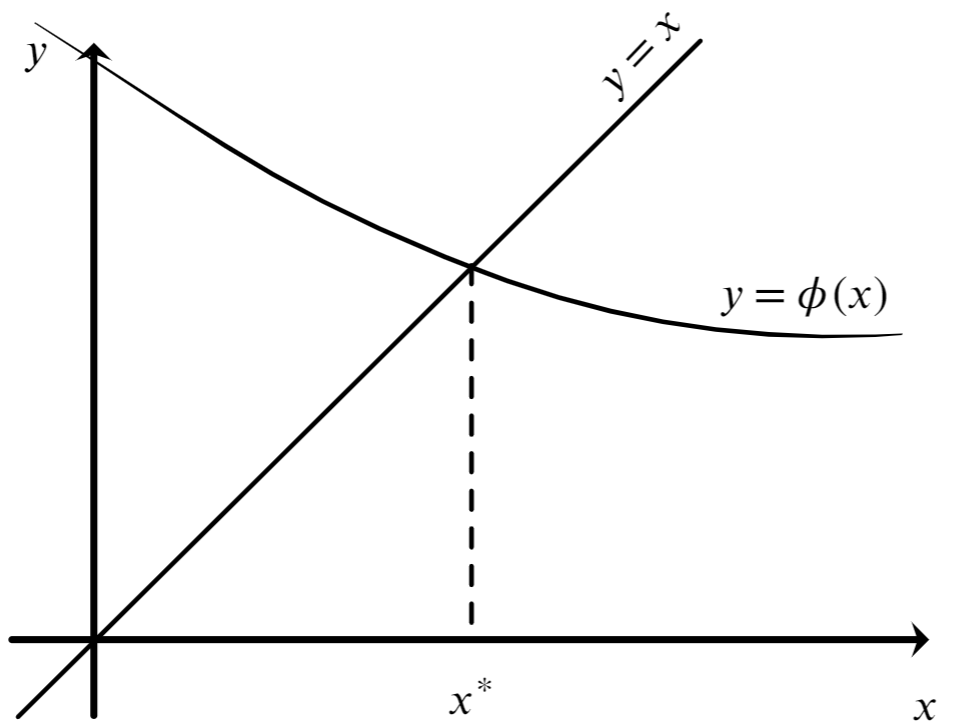
\includegraphics[scale=0.4]{img1.png}\] Таким
образом, после процедуры отделения корней мы находим начальное
приближение \(x^0\) в окрестности корня \(x^*\). И по найденному
начальному приближению строится итерационная
последовательность, которая и называется
\textbf{методом простой итерации.} Мы
должны обеспечить сходимость этого итерационного процесса. Сформулируем для этого теорему.

\begin{theorem}
        [о сходимости метода простой итерации]
        Пусть выполняются следующие условия:\begin{enumerate}
            \item функция $\varphi(x)$ определена на отрезке $$|x - x^0| \leq \delta,$$ непрерывна на нем и удовлетворяет условию Липшица с постоянным коэффициентом меньше единицы, то есть $\forall x, \widetilde{x}$ $$|\varphi(x) - \varphi(\widetilde{x})| \leq q |x - \widetilde{x}| ,\quad 0 \leq q < 1;$$
            \item для начального приближения $x^0$ верно неравенство $$|x^0 - \varphi(x^0)| \leq m;$$
            \item числа $\delta, q, m$ удовлетворяют условию $$\dfrac{m}{1-q}\leq \delta. $$
        \end{enumerate}
        Тогда \begin{enumerate}
            \item уравнение $(1)$ в области $(3)$ имеет решение;
            \item последовательность $x^k$ построенная по правилу $(2)$ принадлежит отрезку $[x^0 - \delta, x^0 + \delta]$, является сходящейся и ее предел удовлетворяет уравнению $(1)$: $$x^k \xrightarrow[k\to \infty]{} x^*;$$
            \item скорость сходимости $x^k$ к $x^*$ оценивается неравенством $$|x^* - x^k| \leq \dfrac{m}{1- q}q^k,\ k = 1,2,\ldots $$
        \end{enumerate}
        Также эта теорема может называется \textbf{методом сжимающих отображений}.
    \end{theorem}

\textbf{Замечание.} \begin{enumerate}
    \item Так как сходимость метода простых итераций возможна при сжимающем
        отображении, то условие \(|\varphi'(x)|<1\) является определяющим при
        приведении исходного уравнения к каноническому виду.
        \textbackslash\textbackslash{} Наиболее универсальными способом
        приведения к каноническому виду является преобразование
        \[x = \underbrace{x+f(x)}_{\varphi(x)},\] но нам необходимо выполнение
        условия \(|\varphi'(x)|<1\). Поэтому мы вводим параметр \(\psi(x)\),
        выбираемый таким образом, чтобы обеспечить сходимость:
        \[x = \underbrace{x+\psi(x)f(x)}_{\varphi(x)},\] Параметр \(\psi(x)\)
        должен быть непрерывным и \(\psi(x^*)\ne 0.\) Самый простой вариант ---
        взять постоянную функцию \(\psi(x)=\operatorname{const}\) и подобрать
        эту константу из условия \(|\varphi'(x)|<1\).
    \end{enumerate}
        

Рассмотрим условие
\[|\varphi'{(x)}| < 1.\]
Приведение к каноническому виду выполним следующим образом:
\[x = x + \psi{(x)}f(x) = \varphi{(x)},\]
где \(\psi{(x)}\) проще всего принять за const, которую подберем из
неравенства
\[|\varphi'{(x)}| < 1,\]
откуда
\[-1 < \varphi'{(x)} < 1,\]
\[-1 < 1 + \psi{(x)}f'(x) < 1,\]
\[-\frac{2}{f(x)} < \psi{(x)} < 0.\]
Пусть \(M = max{(f'(x))}\), тогда
\[\frac{2}{M} < \psi{(x)} < 0.\]
Найдем M на отрезке {[}0, 1.5{]}. Так как раньше мы выяснили, что
производная возрастает на этом отрезке, то нам достаточно найти значение
производной на правом конце отрезка.

    \begin{tcolorbox}[breakable, size=fbox, boxrule=1pt, pad at break*=1mm,colback=cellbackground, colframe=cellborder]
\prompt{In}{incolor}{19}{\boxspacing}
\begin{Verbatim}[commandchars=\\\{\}]
\PY{n}{f\PYZus{}derivative}\PY{p}{(}\PY{l+m+mf}{1.5}\PY{p}{)}

\PY{n}{M}
\end{Verbatim}
\end{tcolorbox}

            \begin{tcolorbox}[breakable, size=fbox, boxrule=.5pt, pad at break*=1mm, opacityfill=0]
\prompt{Out}{outcolor}{19}{\boxspacing}
\begin{Verbatim}[commandchars=\\\{\}]
43.708114183396475
\end{Verbatim}
\end{tcolorbox}
        
    \begin{tcolorbox}[breakable, size=fbox, boxrule=1pt, pad at break*=1mm,colback=cellbackground, colframe=cellborder]
\prompt{In}{incolor}{20}{\boxspacing}
\begin{Verbatim}[commandchars=\\\{\}]
\PY{o}{\PYZhy{}}\PY{l+m+mi}{2}\PY{o}{/}\PY{n}{f\PYZus{}derivative}\PY{p}{(}\PY{l+m+mf}{1.5}\PY{p}{)}
\end{Verbatim}
\end{tcolorbox}

            \begin{tcolorbox}[breakable, size=fbox, boxrule=.5pt, pad at break*=1mm, opacityfill=0]
\prompt{Out}{outcolor}{20}{\boxspacing}
\begin{Verbatim}[commandchars=\\\{\}]
-0.008719979976090307
\end{Verbatim}
\end{tcolorbox}
        
    Получаем, что \(\psi{(x)} \in [-0.008719979976090307, 0]\). Пусть
\(\psi{(x)}= -0.008\), тогда

\[\varphi{(x)} = x - 0.008f(x).\]

Возьмем \(x_0 = 0.75\), тогда \(\delta = 0.75\).

Найдем \(x_1\).

    \begin{tcolorbox}[breakable, size=fbox, boxrule=1pt, pad at break*=1mm,colback=cellbackground, colframe=cellborder]
\prompt{In}{incolor}{21}{\boxspacing}
\begin{Verbatim}[commandchars=\\\{\}]
\PY{k}{def} \PY{n+nf}{phi}\PY{p}{(}\PY{n}{x}\PY{p}{)}\PY{p}{:}
    \PY{k}{return} \PY{n}{x} \PY{o}{\PYZhy{}} \PY{l+m+mf}{0.008}\PY{o}{*}\PY{n}{f}\PY{p}{(}\PY{n}{x}\PY{p}{)}

\PY{n}{x\PYZus{}0} \PY{o}{=} \PY{l+m+mf}{0.75}

\PY{n}{x\PYZus{}1} \PY{o}{=} \PY{n}{phi}\PY{p}{(}\PY{n}{x\PYZus{}0}\PY{p}{)}

\PY{n}{x\PYZus{}1}
\end{Verbatim}
\end{tcolorbox}

            \begin{tcolorbox}[breakable, size=fbox, boxrule=.5pt, pad at break*=1mm, opacityfill=0]
\prompt{Out}{outcolor}{21}{\boxspacing}
\begin{Verbatim}[commandchars=\\\{\}]
0.7557287075537045
\end{Verbatim}
\end{tcolorbox}
        
    Теперь найдем \(m\) из неравенства

\[|x_0-x_1|\leq m.\]

    \begin{tcolorbox}[breakable, size=fbox, boxrule=1pt, pad at break*=1mm,colback=cellbackground, colframe=cellborder]
\prompt{In}{incolor}{22}{\boxspacing}
\begin{Verbatim}[commandchars=\\\{\}]
\PY{n}{m} \PY{o}{=} \PY{n+nb}{abs}\PY{p}{(}\PY{n}{x\PYZus{}0} \PY{o}{\PYZhy{}} \PY{n}{x\PYZus{}1}\PY{p}{)}

\PY{n}{m}
\end{Verbatim}
\end{tcolorbox}

            \begin{tcolorbox}[breakable, size=fbox, boxrule=.5pt, pad at break*=1mm, opacityfill=0]
\prompt{Out}{outcolor}{22}{\boxspacing}
\begin{Verbatim}[commandchars=\\\{\}]
0.005728707553704471
\end{Verbatim}
\end{tcolorbox}
        
    Найдем коэффициент Липшица из неравенства.

    \begin{tcolorbox}[breakable, size=fbox, boxrule=1pt, pad at break*=1mm,colback=cellbackground, colframe=cellborder]
\prompt{In}{incolor}{23}{\boxspacing}
\begin{Verbatim}[commandchars=\\\{\}]
\PY{n}{q} \PY{o}{=} \PY{l+m+mi}{1} \PY{o}{\PYZhy{}} \PY{n}{f\PYZus{}derivative}\PY{p}{(}\PY{l+m+mi}{1}\PY{p}{)}

\PY{n}{q}
\end{Verbatim}
\end{tcolorbox}

            \begin{tcolorbox}[breakable, size=fbox, boxrule=.5pt, pad at break*=1mm, opacityfill=0]
\prompt{Out}{outcolor}{23}{\boxspacing}
\begin{Verbatim}[commandchars=\\\{\}]
-0.9446547290330596
\end{Verbatim}
\end{tcolorbox}
        
    Проверим выполнение последнего условия

\[\frac{m}{1-q}<\delta.\]

    \begin{tcolorbox}[breakable, size=fbox, boxrule=1pt, pad at break*=1mm,colback=cellbackground, colframe=cellborder]
\prompt{In}{incolor}{24}{\boxspacing}
\begin{Verbatim}[commandchars=\\\{\}]
\PY{n}{delta} \PY{o}{=} \PY{l+m+mf}{0.75}

\PY{n}{m}\PY{o}{/}\PY{p}{(}\PY{l+m+mi}{1}\PY{o}{\PYZhy{}}\PY{n}{q}\PY{p}{)} \PY{o}{\PYZlt{}} \PY{n}{delta}
\end{Verbatim}
\end{tcolorbox}

            \begin{tcolorbox}[breakable, size=fbox, boxrule=.5pt, pad at break*=1mm, opacityfill=0]
\prompt{Out}{outcolor}{24}{\boxspacing}
\begin{Verbatim}[commandchars=\\\{\}]
True
\end{Verbatim}
\end{tcolorbox}
        
    Так как условия теоремы выполняются, то можно сделать вывод, что метод
простой итерации на отрезке \([1, 1.5]\) сходится. Реализуем метод
простой итерации программно.

    \begin{tcolorbox}[breakable, size=fbox, boxrule=1pt, pad at break*=1mm,colback=cellbackground, colframe=cellborder]
\prompt{In}{incolor}{25}{\boxspacing}
\begin{Verbatim}[commandchars=\\\{\}]
\PY{k}{def} \PY{n+nf}{simple\PYZus{}iteration\PYZus{}method}\PY{p}{(}\PY{n}{x0}\PY{p}{,} \PY{n}{epsilon}\PY{p}{,} \PY{n}{max\PYZus{}iterations}\PY{p}{)}\PY{p}{:}
    \PY{n}{x\PYZus{}prev} \PY{o}{=} \PY{n}{x0}
    \PY{n}{x\PYZus{}next} \PY{o}{=} \PY{n}{phi}\PY{p}{(}\PY{n}{x\PYZus{}prev}\PY{p}{)}
    \PY{n}{iterations} \PY{o}{=} \PY{l+m+mi}{1}

    \PY{n}{x\PYZus{}k} \PY{o}{=} \PY{p}{[}\PY{p}{]}
    
    \PY{k}{while} \PY{n+nb}{abs}\PY{p}{(}\PY{n}{x\PYZus{}next} \PY{o}{\PYZhy{}} \PY{n}{x\PYZus{}prev}\PY{p}{)} \PY{o}{\PYZgt{}} \PY{n}{epsilon} \PY{o+ow}{and} \PY{n}{iterations} \PY{o}{\PYZlt{}} \PY{n}{max\PYZus{}iterations}\PY{p}{:}
        \PY{n}{x\PYZus{}k}\PY{o}{.}\PY{n}{append}\PY{p}{(}\PY{p}{[}\PY{n}{x\PYZus{}next}\PY{p}{,} \PY{n+nb}{abs}\PY{p}{(}\PY{n}{x\PYZus{}next} \PY{o}{\PYZhy{}} \PY{n}{x\PYZus{}prev}\PY{p}{)}\PY{p}{]}\PY{p}{)}
        
        \PY{n}{x\PYZus{}prev} \PY{o}{=} \PY{n}{x\PYZus{}next}
        \PY{n}{x\PYZus{}next} \PY{o}{=} \PY{n}{phi}\PY{p}{(}\PY{n}{x\PYZus{}prev}\PY{p}{)}
        \PY{n}{iterations} \PY{o}{+}\PY{o}{=} \PY{l+m+mi}{1}
        
    \PY{k}{if} \PY{n}{iterations} \PY{o}{==} \PY{n}{max\PYZus{}iterations}\PY{p}{:}
        \PY{n+nb}{print}\PY{p}{(}\PY{l+s+s2}{\PYZdq{}}\PY{l+s+s2}{Максимальное количество итераций достигнуто!}\PY{l+s+s2}{\PYZdq{}}\PY{p}{)}

    \PY{n}{x\PYZus{}k}\PY{o}{.}\PY{n}{append}\PY{p}{(}\PY{p}{[}\PY{n}{x\PYZus{}next}\PY{p}{,} \PY{n+nb}{abs}\PY{p}{(}\PY{n}{x\PYZus{}next} \PY{o}{\PYZhy{}} \PY{n}{x\PYZus{}prev}\PY{p}{)}\PY{p}{]}\PY{p}{)}
    \PY{k}{return} \PY{n}{x\PYZus{}k}

\PY{n}{epsilon} \PY{o}{=} \PY{l+m+mf}{1e\PYZhy{}6}
\PY{n}{max\PYZus{}iterations} \PY{o}{=} \PY{l+m+mi}{1000}

\PY{n}{root} \PY{o}{=} \PY{n}{simple\PYZus{}iteration\PYZus{}method}\PY{p}{(}\PY{n}{x\PYZus{}0}\PY{p}{,} \PY{n}{epsilon}\PY{p}{,} \PY{n}{max\PYZus{}iterations}\PY{p}{)}
\PY{n+nb}{print}\PY{p}{(}\PY{l+s+s2}{\PYZdq{}}\PY{l+s+s2}{Корень:}\PY{l+s+s2}{\PYZdq{}}\PY{p}{,} \PY{n}{root}\PY{p}{[}\PY{n+nb}{len}\PY{p}{(}\PY{n}{root}\PY{p}{)} \PY{o}{\PYZhy{}} \PY{l+m+mi}{1}\PY{p}{]}\PY{p}{[}\PY{l+m+mi}{0}\PY{p}{]}\PY{p}{)}

\PY{n}{df} \PY{o}{=} \PY{n}{pd}\PY{o}{.}\PY{n}{concat}\PY{p}{(}\PY{p}{[}\PY{n}{df}\PY{p}{,} \PY{n}{pd}\PY{o}{.}\PY{n}{DataFrame}\PY{p}{(}\PY{n}{root}\PY{p}{,} \PY{n}{columns}\PY{o}{=}\PY{p}{[}\PY{p}{(}\PY{l+s+s1}{\PYZsq{}}\PY{l+s+s1}{Метод простой итерации}\PY{l+s+s1}{\PYZsq{}}\PY{p}{,} \PY{l+s+s1}{\PYZsq{}}\PY{l+s+s1}{Решение}\PY{l+s+s1}{\PYZsq{}}\PY{p}{)}\PY{p}{,} \PY{p}{(}\PY{l+s+s1}{\PYZsq{}}\PY{l+s+s1}{Метод простой итерации}\PY{l+s+s1}{\PYZsq{}}\PY{p}{,} \PY{l+s+s1}{\PYZsq{}}\PY{l+s+s1}{Погрешность}\PY{l+s+s1}{\PYZsq{}}\PY{p}{)}\PY{p}{]}\PY{p}{)}\PY{p}{]}\PY{p}{,} \PY{n}{axis}\PY{o}{=}\PY{l+m+mi}{1}\PY{p}{,} \PY{n}{verify\PYZus{}integrity}\PY{o}{=}\PY{k+kc}{True}\PY{p}{)}\PY{o}{.}\PY{n}{fillna}\PY{p}{(}\PY{l+s+s1}{\PYZsq{}}\PY{l+s+s1}{\PYZsq{}}\PY{p}{)}
\end{Verbatim}
\end{tcolorbox}

    \begin{Verbatim}[commandchars=\\\{\}]
Корень: 1.1459385397465647
    \end{Verbatim}

    \subsection*{Метод Стеффенсена}

Метод Стеффенсена основывается на том, что мы укажем способ вычисления $x^{k+1}$ через $x^k$ таким образом, чтобы обеспечить квадратичную скорость сходимости. Для увеличения скорости сходимости в данном методе используется преобразование Эйткена.

Пусть мы имеем $x^0$. Берем приближения $$x^1 = \varphi(x^0), \quad x^2 = \varphi(x^1) = \varphi(\varphi(x^0)).$$
Тогда, используя формулу (7), мы можем при $n=1$ получить $$\sigma_1 = \dfrac{x^0x^2 - (x^1)^2}{x^2 - 2x^1 +x^0} = \dfrac{x^0 \varphi(\varphi(x^0)) - (\varphi(x^0))^2}{\varphi(\varphi(x^0)) - 2 \varphi(x^0) + x^0}.$$
Заменим в этой формуле соответствующим образом индексы. В итоге получается итерационная формула, которая получила название \textbf{метод Стеффенсена}
$$x^{k+1} = \dfrac{x^k \varphi(\varphi(x^k)) - (\varphi(x^k))^2}{\varphi(\varphi(x^k)) - 2 \varphi(x^k) + x^k},\ k=0,1,\ldots;\ x^0.$$
Метод Стеффенсена можно трактовать как метод простой итерации примененный к уравнению вида $$x = \Phi(x),$$ где $$\Phi(x) = \dfrac{x \varphi(\varphi(x)) - \varphi^2(x)}{\varphi(\varphi(x)) - 2\varphi(x) + x}.$$ 
Возникает вопрос сходимости метода.
Можно доказать, что функция $\Phi(x)$ вместе со своей производной будет непрерывна в окрестности точки $x^*$, причем $$\lim\limits_{x\to x^*}\Phi(x) = x^*.$$ Если предположить, что функция $\Phi(x^*) = x^*$ (то есть мы доопределяем ее), то $\Phi(x)$ будет непрерывна в точке $x^*$. Кроме того можно утверждать, что $$\Phi'(x^*) = \lim\limits_{x\to x^*}\dfrac{\Phi(x) - \Phi(x^*)}{x - x^*} = 0.$$
Таким образом, можно утверждать, что сходимость метода Стеффенсена будет квадратичной. То есть мы построили метод, обладающий повышенной скоростью сходимости. Но в 2 раза увеличивается объем вычислений, из-за того, что нужно вычислять функцию $\varphi(\varphi(x))$.

Так как метод Стеффенсена является модификацией метода простой итерации,
то сходимость этого метода идентична сходимости метода простой итерации.

Построим функцию $\Phi(x)$.
    \begin{tcolorbox}[breakable, size=fbox, boxrule=1pt, pad at break*=1mm,colback=cellbackground, colframe=cellborder]
\prompt{In}{incolor}{26}{\boxspacing}
\begin{Verbatim}[commandchars=\\\{\}]
\PY{k}{def} \PY{n+nf}{Phi}\PY{p}{(}\PY{n}{x}\PY{p}{)}\PY{p}{:}
    \PY{k}{return} \PY{p}{(}\PY{n}{x} \PY{o}{*} \PY{n}{phi}\PY{p}{(}\PY{n}{phi}\PY{p}{(}\PY{n}{x}\PY{p}{)}\PY{p}{)} \PY{o}{\PYZhy{}} \PY{p}{(}\PY{n}{phi}\PY{p}{(}\PY{n}{x}\PY{p}{)}\PY{p}{)}\PY{o}{*}\PY{o}{*}\PY{l+m+mi}{2}\PY{p}{)} \PY{o}{/} \PY{p}{(}\PY{n}{phi}\PY{p}{(}\PY{n}{phi}\PY{p}{(}\PY{n}{x}\PY{p}{)}\PY{p}{)} \PY{o}{\PYZhy{}} \PY{l+m+mi}{2} \PY{o}{*} \PY{n}{phi}\PY{p}{(}\PY{n}{x}\PY{p}{)} \PY{o}{+} \PY{n}{x}\PY{p}{)}
\end{Verbatim}
\end{tcolorbox}

    Исходный итерационный процесс сходился, поэтому и новый построенный
итерационный процесс будет также сходящимся. Поэтому перейдем сразу к
программной реализации итерационного процесса.

    \begin{tcolorbox}[breakable, size=fbox, boxrule=1pt, pad at break*=1mm,colback=cellbackground, colframe=cellborder]
\prompt{In}{incolor}{27}{\boxspacing}
\begin{Verbatim}[commandchars=\\\{\}]
\PY{k}{def} \PY{n+nf}{steffensen\PYZus{}method}\PY{p}{(}\PY{n}{x0}\PY{p}{,} \PY{n}{epsilon}\PY{p}{,} \PY{n}{max\PYZus{}iterations}\PY{p}{)}\PY{p}{:}
    \PY{n}{x\PYZus{}prev} \PY{o}{=} \PY{n}{x0}
    \PY{n}{x\PYZus{}next} \PY{o}{=} \PY{n}{Phi}\PY{p}{(}\PY{n}{x0}\PY{p}{)}
    \PY{n}{iterations} \PY{o}{=} \PY{l+m+mi}{1}
    
    \PY{n}{x\PYZus{}k} \PY{o}{=} \PY{p}{[}\PY{p}{]}
    
    \PY{k}{while} \PY{n}{iterations} \PY{o}{\PYZlt{}} \PY{n}{max\PYZus{}iterations}\PY{p}{:}
        \PY{n}{x\PYZus{}prev} \PY{o}{=} \PY{n}{x\PYZus{}next}
        \PY{n}{x\PYZus{}next} \PY{o}{=} \PY{n}{Phi}\PY{p}{(}\PY{n}{x\PYZus{}prev}\PY{p}{)}
        
        \PY{k}{if} \PY{n+nb}{abs}\PY{p}{(}\PY{n}{x\PYZus{}next} \PY{o}{\PYZhy{}} \PY{n}{x\PYZus{}prev}\PY{p}{)} \PY{o}{\PYZlt{}} \PY{n}{epsilon}\PY{p}{:}
            \PY{k}{break}

        \PY{n}{x\PYZus{}k}\PY{o}{.}\PY{n}{append}\PY{p}{(}\PY{p}{[}\PY{n}{x\PYZus{}next}\PY{p}{,} \PY{n+nb}{abs}\PY{p}{(}\PY{n}{x\PYZus{}next} \PY{o}{\PYZhy{}} \PY{n}{x\PYZus{}prev}\PY{p}{)}\PY{p}{]}\PY{p}{)}
        \PY{n}{iterations} \PY{o}{+}\PY{o}{=} \PY{l+m+mi}{1}

    \PY{k}{if} \PY{n}{iterations} \PY{o}{==} \PY{n}{max\PYZus{}iterations}\PY{p}{:}
        \PY{n+nb}{print}\PY{p}{(}\PY{l+s+s2}{\PYZdq{}}\PY{l+s+s2}{Максимальное количество итераций достигнуто!}\PY{l+s+s2}{\PYZdq{}}\PY{p}{)}

    \PY{n}{x\PYZus{}k}\PY{o}{.}\PY{n}{append}\PY{p}{(}\PY{p}{[}\PY{n}{x\PYZus{}next}\PY{p}{,} \PY{n+nb}{abs}\PY{p}{(}\PY{n}{x\PYZus{}next} \PY{o}{\PYZhy{}} \PY{n}{x\PYZus{}prev}\PY{p}{)}\PY{p}{]}\PY{p}{)}
    
    \PY{k}{return} \PY{n}{x\PYZus{}k}

\PY{n}{epsilon} \PY{o}{=} \PY{l+m+mf}{1e\PYZhy{}6}
\PY{n}{max\PYZus{}iterations} \PY{o}{=} \PY{l+m+mi}{100}

\PY{n}{root} \PY{o}{=} \PY{n}{steffensen\PYZus{}method}\PY{p}{(}\PY{n}{x0}\PY{p}{,} \PY{n}{epsilon}\PY{p}{,} \PY{n}{max\PYZus{}iterations}\PY{p}{)}
\PY{n+nb}{print}\PY{p}{(}\PY{l+s+s2}{\PYZdq{}}\PY{l+s+s2}{Корень:}\PY{l+s+s2}{\PYZdq{}}\PY{p}{,} \PY{n}{root}\PY{p}{[}\PY{n+nb}{len}\PY{p}{(}\PY{n}{root}\PY{p}{)} \PY{o}{\PYZhy{}} \PY{l+m+mi}{1}\PY{p}{]}\PY{p}{[}\PY{l+m+mi}{0}\PY{p}{]}\PY{p}{)}

\PY{n}{df} \PY{o}{=} \PY{n}{pd}\PY{o}{.}\PY{n}{concat}\PY{p}{(}\PY{p}{[}\PY{n}{df}\PY{p}{,} \PY{n}{pd}\PY{o}{.}\PY{n}{DataFrame}\PY{p}{(}\PY{n}{root}\PY{p}{,} \PY{n}{columns}\PY{o}{=}\PY{p}{[}\PY{p}{(}\PY{l+s+s1}{\PYZsq{}}\PY{l+s+s1}{Метод Стеффенсена}\PY{l+s+s1}{\PYZsq{}}\PY{p}{,} \PY{l+s+s1}{\PYZsq{}}\PY{l+s+s1}{Решение}\PY{l+s+s1}{\PYZsq{}}\PY{p}{)}\PY{p}{,} \PY{p}{(}\PY{l+s+s1}{\PYZsq{}}\PY{l+s+s1}{Метод Стеффенсена}\PY{l+s+s1}{\PYZsq{}}\PY{p}{,} \PY{l+s+s1}{\PYZsq{}}\PY{l+s+s1}{Погрешность}\PY{l+s+s1}{\PYZsq{}}\PY{p}{)}\PY{p}{]}\PY{p}{)}\PY{p}{]}\PY{p}{,} \PY{n}{axis}\PY{o}{=}\PY{l+m+mi}{1}\PY{p}{,} \PY{n}{verify\PYZus{}integrity}\PY{o}{=}\PY{k+kc}{True}\PY{p}{)}\PY{o}{.}\PY{n}{fillna}\PY{p}{(}\PY{l+s+s1}{\PYZsq{}}\PY{l+s+s1}{\PYZsq{}}\PY{p}{)}
\end{Verbatim}
\end{tcolorbox}

    \begin{Verbatim}[commandchars=\\\{\}]
Корень: 1.145964910905985
    \end{Verbatim}

    \subsection*{Метод Чебышева третьего порядка}

Идея метода базируется на способе построения итерационного процесса
таким образом, чтобы обеспечить обращение в ноль производных от функции
\(\varphi(x)\) в точке \(x^*\), то есть мы берем уравнение
\[x = \varphi(x)\] и стараемся построить метод, у которого максимальное
количество производных обращается в ноль в точке \(x^*\). Для этого
функцию \(\varphi(x)\) запишем в виде
\[\varphi(x) = x+ \psi_1(x) f(x) + \psi_2(x)f^2(x) + \ldots + \psi_{n-1}(x)f^{n-1}(x),\]
где \(f(x)\) --- это исходная функция, для которой мы ищем корни.
Требуется выбрать функции \(\psi_1(x),\ldots, \psi_{n-1}(x)\) так, чтобы
\[\varphi^{(j)}(x)\Big|_{f(x)=0} = 0,\quad j=1,2,\ldots,n-1 \]
Рассмотрим условие на первую производную \begin{multline*}
    \varphi'(x)\Big|_{f(x) = 0} = 1 + \psi_1'(x)f(x) + \psi_1(x) f'(x) + \psi_2'(x) f^2(x) + 2\psi_2(x) f(x) f'(x) + \ldots \Big|_{f(x) = 0}=\\=1 + \psi_1(x) f'(x) \Big|_{f(x) = 0} = 0.
\end{multline*} Аналогичным образом мы можем записать вторую производную
\[\varphi''(x)\Big|_{f(x) = 0} = 2\psi_1' f'(x) + \psi_1(x) f''(x) + 2\psi_2(x) (f'(x))^2 \Big|_{f(x) = 0} = 0.\]
Из условия \(\varphi'(x)\Big|_{f(x) = 0}=0\) следует, что функция
\[\psi_1(x) = -\dfrac{1}{f'(x)}.\] Отсюда
\[\varphi(x) = x + \Big(-\dfrac{1}{f'(x)}\Big)f(x),\] то есть мы пришли
к методу Ньютона, итерационному процессу второго порядка. Из условия,
что \(\varphi''(x)\Big|_{f(x) = 0}=0\), применяя простые арифметические
действия, мы можем получить \[\psi_2(x) = -\dfrac{f''(x)}{2(f'(x))^3}.\]
Учитывая выражения для \(\psi_1\) и \(\psi_2\) мы модем построить
итерационный процесс третьего порядка с кубической скоростью сходимости
\[x^{k+1} = x^k - \dfrac{f(x^k)}{f'(x^k)} - \dfrac{f^2(x^k)f''(x^k)}{2(f'(x^k))^3}\]
и будем называть эту формулу \textbf{методом Чебышева}. В этом методе мы
также увеличиваем количество операций, так как необходимо вычислять
значения \(f(x), f'(x), f''(x)\).

Поскольку метод Чебышева является модификацией метода простой итерации,
то его сходимость на отрезке \([1, 1.5]\) вытекает их сходимости метода
простой итерации, начальное приближение мы также уже выбрали, поэтому
сразу перейдем к программной реализации.

    \begin{tcolorbox}[breakable, size=fbox, boxrule=1pt, pad at break*=1mm,colback=cellbackground, colframe=cellborder]
\prompt{In}{incolor}{28}{\boxspacing}
\begin{Verbatim}[commandchars=\\\{\}]
\PY{k}{def} \PY{n+nf}{phi}\PY{p}{(}\PY{n}{x}\PY{p}{)}\PY{p}{:}
    \PY{k}{return} \PY{n}{x} \PY{o}{\PYZhy{}} \PY{n}{f}\PY{p}{(}\PY{n}{x}\PY{p}{)} \PY{o}{/} \PY{n}{f\PYZus{}derivative}\PY{p}{(}\PY{n}{x}\PY{p}{)} \PY{o}{\PYZhy{}} \PY{n}{f}\PY{p}{(}\PY{n}{x}\PY{p}{)}\PY{o}{*}\PY{o}{*}\PY{l+m+mi}{2} \PY{o}{*} \PY{n}{f\PYZus{}second\PYZus{}derivative}\PY{p}{(}\PY{n}{x}\PY{p}{)} \PY{o}{/} \PY{p}{(}\PY{l+m+mi}{2} \PY{o}{*} \PY{n}{f\PYZus{}derivative}\PY{p}{(}\PY{n}{x}\PY{p}{)}\PY{o}{*}\PY{o}{*}\PY{l+m+mi}{3}\PY{p}{)}

\PY{k}{def} \PY{n+nf}{chebyshev\PYZus{}method}\PY{p}{(}\PY{n}{x0}\PY{p}{,} \PY{n}{epsilon}\PY{p}{,} \PY{n}{max\PYZus{}iterations}\PY{p}{)}\PY{p}{:}
    \PY{n}{x\PYZus{}prev} \PY{o}{=} \PY{n}{x0}
    \PY{n}{x\PYZus{}next} \PY{o}{=} \PY{n}{phi}\PY{p}{(}\PY{n}{x\PYZus{}prev}\PY{p}{)}
    \PY{n}{iterations} \PY{o}{=} \PY{l+m+mi}{1}

    \PY{n}{x\PYZus{}k} \PY{o}{=} \PY{p}{[}\PY{p}{]}
    
    \PY{k}{while} \PY{n}{iterations} \PY{o}{\PYZlt{}} \PY{n}{max\PYZus{}iterations}\PY{p}{:}
        \PY{n}{x\PYZus{}prev} \PY{o}{=} \PY{n}{x\PYZus{}next}
        \PY{n}{x\PYZus{}next} \PY{o}{=} \PY{n}{phi}\PY{p}{(}\PY{n}{x\PYZus{}prev}\PY{p}{)}
        
        \PY{k}{if} \PY{n+nb}{abs}\PY{p}{(}\PY{n}{x\PYZus{}next} \PY{o}{\PYZhy{}} \PY{n}{x\PYZus{}prev}\PY{p}{)} \PY{o}{\PYZlt{}} \PY{n}{epsilon}\PY{p}{:}
            \PY{k}{break}
            
        \PY{n}{x\PYZus{}k}\PY{o}{.}\PY{n}{append}\PY{p}{(}\PY{p}{[}\PY{n}{x\PYZus{}next}\PY{p}{,} \PY{n+nb}{abs}\PY{p}{(}\PY{n}{x\PYZus{}next} \PY{o}{\PYZhy{}} \PY{n}{x\PYZus{}prev}\PY{p}{)}\PY{p}{]}\PY{p}{)}
        \PY{n}{iterations} \PY{o}{+}\PY{o}{=} \PY{l+m+mi}{1}

    \PY{k}{if} \PY{n}{iterations} \PY{o}{==} \PY{n}{max\PYZus{}iterations}\PY{p}{:}
        \PY{n+nb}{print}\PY{p}{(}\PY{l+s+s2}{\PYZdq{}}\PY{l+s+s2}{Максимальное количество итераций достигнуто!}\PY{l+s+s2}{\PYZdq{}}\PY{p}{)}

    \PY{n}{x\PYZus{}k}\PY{o}{.}\PY{n}{append}\PY{p}{(}\PY{p}{[}\PY{n}{x\PYZus{}next}\PY{p}{,} \PY{n+nb}{abs}\PY{p}{(}\PY{n}{x\PYZus{}next} \PY{o}{\PYZhy{}} \PY{n}{x\PYZus{}prev}\PY{p}{)}\PY{p}{]}\PY{p}{)}
    
    \PY{k}{return} \PY{n}{x\PYZus{}k}

\PY{k}{def} \PY{n+nf}{f}\PY{p}{(}\PY{n}{x}\PY{p}{)}\PY{p}{:}
    \PY{k}{return} \PY{n}{x}\PY{o}{*}\PY{o}{*}\PY{p}{(}\PY{l+m+mi}{1}\PY{o}{/}\PY{l+m+mi}{3}\PY{p}{)}\PY{o}{*}\PY{n}{math}\PY{o}{.}\PY{n}{tan}\PY{p}{(}\PY{n}{x}\PY{p}{)} \PY{o}{\PYZhy{}} \PY{n}{x}\PY{o}{*}\PY{o}{*}\PY{l+m+mi}{2} \PY{o}{\PYZhy{}} \PY{l+m+mi}{1}

\PY{n}{epsilon} \PY{o}{=} \PY{l+m+mf}{1e\PYZhy{}6}
\PY{n}{max\PYZus{}iterations} \PY{o}{=} \PY{l+m+mi}{100}

\PY{n}{root} \PY{o}{=} \PY{n}{chebyshev\PYZus{}method}\PY{p}{(}\PY{n}{x0}\PY{p}{,} \PY{n}{epsilon}\PY{p}{,} \PY{n}{max\PYZus{}iterations}\PY{p}{)}
\PY{n+nb}{print}\PY{p}{(}\PY{l+s+s2}{\PYZdq{}}\PY{l+s+s2}{Корень:}\PY{l+s+s2}{\PYZdq{}}\PY{p}{,} \PY{n}{root}\PY{p}{[}\PY{n+nb}{len}\PY{p}{(}\PY{n}{root}\PY{p}{)} \PY{o}{\PYZhy{}} \PY{l+m+mi}{1}\PY{p}{]}\PY{p}{[}\PY{l+m+mi}{0}\PY{p}{]}\PY{p}{)}

\PY{n}{df} \PY{o}{=} \PY{n}{pd}\PY{o}{.}\PY{n}{concat}\PY{p}{(}\PY{p}{[}\PY{n}{df}\PY{p}{,} \PY{n}{pd}\PY{o}{.}\PY{n}{DataFrame}\PY{p}{(}\PY{n}{root}\PY{p}{,} \PY{n}{columns}\PY{o}{=}\PY{p}{[}\PY{p}{(}\PY{l+s+s1}{\PYZsq{}}\PY{l+s+s1}{Метод Чебышева}\PY{l+s+s1}{\PYZsq{}}\PY{p}{,} \PY{l+s+s1}{\PYZsq{}}\PY{l+s+s1}{Решение}\PY{l+s+s1}{\PYZsq{}}\PY{p}{)}\PY{p}{,} \PY{p}{(}\PY{l+s+s1}{\PYZsq{}}\PY{l+s+s1}{Метод Чебышева}\PY{l+s+s1}{\PYZsq{}}\PY{p}{,} \PY{l+s+s1}{\PYZsq{}}\PY{l+s+s1}{Погрешность}\PY{l+s+s1}{\PYZsq{}}\PY{p}{)}\PY{p}{]}\PY{p}{)}\PY{p}{]}\PY{p}{,} \PY{n}{axis}\PY{o}{=}\PY{l+m+mi}{1}\PY{p}{,} \PY{n}{verify\PYZus{}integrity}\PY{o}{=}\PY{k+kc}{True}\PY{p}{)}\PY{o}{.}\PY{n}{fillna}\PY{p}{(}\PY{l+s+s1}{\PYZsq{}}\PY{l+s+s1}{\PYZsq{}}\PY{p}{)}
\end{Verbatim}
\end{tcolorbox}

    \begin{Verbatim}[commandchars=\\\{\}]
Корень: 1.1459643670645736
    \end{Verbatim}

    \subsection*{Сравнительная характеристика методов}

На протежении выполнения лабораторной работы заполнялся DataFrame для
наглядности происходящего. Рассмотрим его.

    \begin{tcolorbox}[breakable, size=fbox, boxrule=1pt, pad at break*=1mm,colback=cellbackground, colframe=cellborder]
\prompt{In}{incolor}{29}{\boxspacing}
\begin{Verbatim}[commandchars=\\\{\}]
\PY{n}{df}
\end{Verbatim}
\end{tcolorbox}

            \begin{tcolorbox}[breakable, size=fbox, boxrule=.5pt, pad at break*=1mm, opacityfill=0]
\prompt{Out}{outcolor}{29}{\boxspacing}
\begin{Verbatim}[commandchars=\\\{\}]
    (Метод Ньютона, Решение) (Метод Ньютона, Погрешность)  \textbackslash{}
0                 1.15454128                   0.04545872
1                 1.14619221                   0.00834908
2                 1.14596453                   0.00022768
3                 1.14596437                   0.00000016
4
..                       {\ldots}                          {\ldots}
294
295
296
297
298

     (Метод простой итерации, Решение)  (Метод простой итерации, Погрешность)  \textbackslash{}
0                           0.75572871                             0.00572871
1                           0.76143083                             0.00570212
2                           0.76710587                             0.00567503
3                           0.77275329                             0.00564742
4                           0.77837256                             0.00561928
..                                 {\ldots}                                    {\ldots}
294                         1.14593442                             0.00000113
295                         1.14593551                             0.00000109
296                         1.14593656                             0.00000105
297                         1.14593757                             0.00000101
298                         1.14593854                             0.00000097

    (Метод Стеффенсена, Решение) (Метод Стеффенсена, Погрешность)  \textbackslash{}
0                     1.14616572                       0.00801378
1                     1.14596449                       0.00020123
2                     1.14596343                       0.00000106
3                     1.14596445                       0.00000102
4                     1.14596491                       0.00000046
..                           {\ldots}                              {\ldots}
294
295
296
297
298

    (Метод Чебышева, Решение) (Метод Чебышева, Погрешность)
0                  1.14596441                    0.00157775
1                  1.14596437                    0.00000005
2
3
4
..                        {\ldots}                           {\ldots}
294
295
296
297
298

[299 rows x 8 columns]
\end{Verbatim}
\end{tcolorbox}
        
    Видно, что каждый метод получил решение с нужной нам точностью до шести
знаков. Однако методу простой итерации понадобилось 299 итераций, что
гораздо медленней, чем у остальных методов, что логично, так как он
является наиболее простым из итерационных и обладает линейно скоростью
сходимости. Наиболее быстрым оказался метод Чебышева, что было очевидно,
так как он имеет кубическую скорость сходимости, который справился всего
за 2 итерации, он же оказался и самым точным. На втором месте по
точности стал метод Ньютона, имеющий квадратичную скорость сходимости.
На третьем месте стал метод Стеффенсена, который также обладает
квадратичной скоростью сходимости. То, что метод Стеффенсена оказался
немного медленней можно объяснить особенностями нашей задачи.

    \section*{Задача 2}

Найти с точностью \({\epsilon = 10^{-6}}\) наибольший по модулю корень
уравнения
\[\sum_{i=0}^na_ix^i=0,\]
где векто коэффицирента \(a\) есть решение системы линейных
алгебраических уравнений \(Aa=f\) с
\[  A = \begin{bmatrix}
        15 & -2 & 3.5 & 1 & -0.1 \\ 
        1 & -8 & -3.1 & 1 & 2.3 \\ 
        -1 & 3 & 30 & 2 & 4.6 \\ 
        0 & 0.1 & 2 & 15 & 2 \\ 
        1 & -2 & 0.4 & 3.2 & -17 
    \end{bmatrix}, \quad
    f = \begin{bmatrix}1 \\ 0 \\ 20 \\ -3 \\ 5 \end{bmatrix} \]
    Первым делом найдем решение системы \(Aa=f\). Сделаем это одним из
реализованных в прошлом методом, а именно методом релаксации.

    \begin{tcolorbox}[breakable, size=fbox, boxrule=1pt, pad at break*=1mm,colback=cellbackground, colframe=cellborder]
\prompt{In}{incolor}{30}{\boxspacing}
\begin{Verbatim}[commandchars=\\\{\}]
\PY{n}{A} \PY{o}{=} \PY{n}{np}\PY{o}{.}\PY{n}{array}\PY{p}{(}\PY{p}{[}\PY{p}{[}\PY{l+m+mi}{15}\PY{p}{,} \PY{o}{\PYZhy{}}\PY{l+m+mi}{2}\PY{p}{,} \PY{l+m+mf}{3.5}\PY{p}{,} \PY{l+m+mi}{1}\PY{p}{,} \PY{o}{\PYZhy{}}\PY{l+m+mf}{0.1}\PY{p}{]}\PY{p}{,}
              \PY{p}{[}\PY{l+m+mi}{1}\PY{p}{,} \PY{o}{\PYZhy{}}\PY{l+m+mi}{8}\PY{p}{,} \PY{o}{\PYZhy{}}\PY{l+m+mf}{3.1}\PY{p}{,} \PY{l+m+mi}{1}\PY{p}{,} \PY{l+m+mf}{2.3}\PY{p}{]}\PY{p}{,}
              \PY{p}{[}\PY{o}{\PYZhy{}}\PY{l+m+mi}{1}\PY{p}{,} \PY{l+m+mi}{3}\PY{p}{,} \PY{l+m+mi}{30}\PY{p}{,} \PY{l+m+mi}{2}\PY{p}{,} \PY{l+m+mf}{4.6}\PY{p}{]}\PY{p}{,}
              \PY{p}{[}\PY{l+m+mi}{0}\PY{p}{,} \PY{l+m+mf}{0.1}\PY{p}{,} \PY{l+m+mi}{2}\PY{p}{,} \PY{l+m+mi}{15}\PY{p}{,} \PY{l+m+mi}{2}\PY{p}{]}\PY{p}{,}
              \PY{p}{[}\PY{l+m+mi}{1}\PY{p}{,} \PY{o}{\PYZhy{}}\PY{l+m+mi}{2}\PY{p}{,} \PY{l+m+mf}{0.4}\PY{p}{,} \PY{l+m+mf}{3.2}\PY{p}{,} \PY{o}{\PYZhy{}}\PY{l+m+mi}{17}\PY{p}{]}\PY{p}{]}\PY{p}{)}

\PY{n}{n} \PY{o}{=} \PY{n+nb}{len}\PY{p}{(}\PY{n}{A}\PY{p}{[}\PY{l+m+mi}{0}\PY{p}{]}\PY{p}{)}

\PY{n}{b} \PY{o}{=} \PY{n}{np}\PY{o}{.}\PY{n}{array}\PY{p}{(}\PY{p}{[}\PY{l+m+mi}{1}\PY{p}{,} \PY{l+m+mi}{0}\PY{p}{,} \PY{l+m+mi}{20}\PY{p}{,} \PY{o}{\PYZhy{}}\PY{l+m+mi}{3}\PY{p}{,} \PY{l+m+mi}{5}\PY{p}{]}\PY{p}{)}

\PY{k}{def} \PY{n+nf}{sum1}\PY{p}{(}\PY{n}{A}\PY{p}{,} \PY{n}{x}\PY{p}{,} \PY{n}{i}\PY{p}{,} \PY{n}{n}\PY{p}{)}\PY{p}{:}
    \PY{n}{s} \PY{o}{=} \PY{l+m+mi}{0}

    \PY{k}{for} \PY{n}{j} \PY{o+ow}{in} \PY{n+nb}{range}\PY{p}{(}\PY{n}{i}\PY{p}{)}\PY{p}{:}
        \PY{n}{s} \PY{o}{+}\PY{o}{=} \PY{n}{A}\PY{p}{[}\PY{n}{i}\PY{p}{,} \PY{n}{j}\PY{p}{]} \PY{o}{*} \PY{n}{x}\PY{p}{[}\PY{n}{j}\PY{p}{]}

    \PY{k}{return} \PY{n}{s}

\PY{k}{def} \PY{n+nf}{sum2}\PY{p}{(}\PY{n}{A}\PY{p}{,} \PY{n}{x}\PY{p}{,} \PY{n}{i}\PY{p}{,} \PY{n}{n}\PY{p}{)}\PY{p}{:}
    \PY{n}{s} \PY{o}{=} \PY{l+m+mi}{0}
    
    \PY{k}{for} \PY{n}{j} \PY{o+ow}{in} \PY{n+nb}{range}\PY{p}{(}\PY{n}{i} \PY{o}{+} \PY{l+m+mi}{1}\PY{p}{,} \PY{n}{n}\PY{p}{)}\PY{p}{:}
        \PY{n}{s} \PY{o}{+}\PY{o}{=} \PY{n}{A}\PY{p}{[}\PY{n}{i}\PY{p}{,} \PY{n}{j}\PY{p}{]} \PY{o}{*} \PY{n}{x}\PY{p}{[}\PY{n}{j}\PY{p}{]}
        
    \PY{k}{return} \PY{n}{s}

\PY{k}{def} \PY{n+nf}{relaxation\PYZus{}method}\PY{p}{(}\PY{n}{A}\PY{p}{,} \PY{n}{b}\PY{p}{,} \PY{n}{n}\PY{p}{,} \PY{n}{epsilon} \PY{o}{=} \PY{l+m+mf}{1e\PYZhy{}4}\PY{p}{,} \PY{n}{max\PYZus{}iterations} \PY{o}{=} \PY{l+m+mi}{300}\PY{p}{,} \PY{n}{w} \PY{o}{=} \PY{l+m+mf}{1.5}\PY{p}{)}\PY{p}{:}
    \PY{n}{x} \PY{o}{=} \PY{n}{np}\PY{o}{.}\PY{n}{zeros}\PY{p}{(}\PY{p}{(}\PY{n}{n}\PY{p}{,} \PY{l+m+mi}{1}\PY{p}{)}\PY{p}{)}

    \PY{k}{for} \PY{n}{\PYZus{}} \PY{o+ow}{in} \PY{n+nb}{range}\PY{p}{(}\PY{n}{max\PYZus{}iterations}\PY{p}{)}\PY{p}{:}
        \PY{n}{x\PYZus{}new} \PY{o}{=} \PY{n}{np}\PY{o}{.}\PY{n}{zeros\PYZus{}like}\PY{p}{(}\PY{n}{x}\PY{p}{)}

        \PY{k}{for} \PY{n}{i} \PY{o+ow}{in} \PY{n+nb}{range}\PY{p}{(}\PY{n}{n}\PY{p}{)}\PY{p}{:}
            \PY{n}{x\PYZus{}new}\PY{p}{[}\PY{n}{i}\PY{p}{]} \PY{o}{=} \PY{p}{(}\PY{l+m+mi}{1} \PY{o}{\PYZhy{}} \PY{n}{w}\PY{p}{)} \PY{o}{*} \PY{n}{x}\PY{p}{[}\PY{n}{i}\PY{p}{]} \PY{o}{+} \PY{p}{(}\PY{n}{w} \PY{o}{/} \PY{n}{A}\PY{p}{[}\PY{n}{i}\PY{p}{,} \PY{n}{i}\PY{p}{]}\PY{p}{)} \PY{o}{*} \PY{p}{(}\PY{n}{b}\PY{p}{[}\PY{n}{i}\PY{p}{]} \PY{o}{\PYZhy{}} \PY{n}{sum1}\PY{p}{(}\PY{n}{A}\PY{p}{,} \PY{n}{x\PYZus{}new}\PY{p}{,} \PY{n}{i}\PY{p}{,} \PY{n}{n}\PY{p}{)} \PY{o}{\PYZhy{}} \PY{n}{sum2}\PY{p}{(}\PY{n}{A}\PY{p}{,} \PY{n}{x}\PY{p}{,} \PY{n}{i}\PY{p}{,} \PY{n}{n}\PY{p}{)}\PY{p}{)}

        \PY{k}{if} \PY{n}{np}\PY{o}{.}\PY{n}{max}\PY{p}{(}\PY{n}{np}\PY{o}{.}\PY{n}{abs}\PY{p}{(}\PY{n}{x\PYZus{}new} \PY{o}{\PYZhy{}} \PY{n}{x}\PY{p}{)}\PY{p}{)} \PY{o}{\PYZlt{}} \PY{n}{epsilon}\PY{p}{:}
            \PY{k}{return} \PY{n}{x\PYZus{}new}

        \PY{n}{x} \PY{o}{=} \PY{n}{x\PYZus{}new}

    \PY{k}{return} \PY{n}{x}

\PY{n}{a} \PY{o}{=} \PY{n}{relaxation\PYZus{}method}\PY{p}{(}\PY{n}{A}\PY{p}{,} \PY{n}{b}\PY{p}{,} \PY{n}{n}\PY{p}{)}

\PY{n+nb}{print}\PY{p}{(}\PY{n}{a}\PY{p}{)}
\end{Verbatim}
\end{tcolorbox}

    \begin{Verbatim}[commandchars=\\\{\}]
[[-0.15378659]
 [-0.4301327 ]
 [ 0.76546924]
 [-0.26136514]
 [-0.28375325]]
    \end{Verbatim}

    Получили коэффициенты для нашего многочлена. Определим его.

    \begin{tcolorbox}[breakable, size=fbox, boxrule=1pt, pad at break*=1mm,colback=cellbackground, colframe=cellborder]
\prompt{In}{incolor}{31}{\boxspacing}
\begin{Verbatim}[commandchars=\\\{\}]
\PY{k}{def} \PY{n+nf}{P}\PY{p}{(}\PY{n}{x}\PY{p}{)}\PY{p}{:}
    \PY{n}{p} \PY{o}{=} \PY{l+m+mi}{0}
    \PY{n}{n} \PY{o}{=} \PY{n+nb}{len}\PY{p}{(}\PY{n}{a}\PY{p}{)}
    
    \PY{k}{for} \PY{n}{i} \PY{o+ow}{in} \PY{n+nb}{range}\PY{p}{(}\PY{n}{n}\PY{p}{)}\PY{p}{:}
        \PY{n}{p} \PY{o}{+}\PY{o}{=} \PY{n}{x}\PY{o}{*}\PY{o}{*}\PY{n}{i} \PY{o}{*} \PY{n+nb}{float}\PY{p}{(}\PY{n}{a}\PY{p}{[}\PY{n}{i}\PY{p}{]}\PY{p}{)}
        
    \PY{k}{return} \PY{n}{p}
\end{Verbatim}
\end{tcolorbox}

    Задачу отыскания наибольшего по модулю корня уравнения можно поделить по
тем же этапам, что и в первой задаче. То есть сначала нам необходимо
решить задачу отделения корней, а затем поиск его приближения с заданной
точностью.

Для того, чтобы понять, есть ли у нашего уравнения действительные корни,
рассмотрим график функции \(P(x)\).

    \begin{tcolorbox}[breakable, size=fbox, boxrule=1pt, pad at break*=1mm,colback=cellbackground, colframe=cellborder]
\prompt{In}{incolor}{32}{\boxspacing}
\begin{Verbatim}[commandchars=\\\{\}]
\PY{n}{x} \PY{o}{=} \PY{n}{np}\PY{o}{.}\PY{n}{linspace}\PY{p}{(}\PY{o}{\PYZhy{}}\PY{l+m+mi}{10}\PY{p}{,} \PY{l+m+mi}{10}\PY{p}{,} \PY{l+m+mi}{1000}\PY{p}{)}

\PY{n}{fig}\PY{p}{,} \PY{n}{ax} \PY{o}{=} \PY{n}{plt}\PY{o}{.}\PY{n}{subplots}\PY{p}{(}\PY{p}{)}

\PY{n}{ax}\PY{o}{.}\PY{n}{plot}\PY{p}{(}\PY{n}{x}\PY{p}{,} \PY{n}{P}\PY{p}{(}\PY{n}{x}\PY{p}{)}\PY{p}{)}
\PY{n}{ax}\PY{o}{.}\PY{n}{plot}\PY{p}{(}\PY{n}{x}\PY{p}{,} \PY{l+m+mi}{0}\PY{o}{*}\PY{n}{x}\PY{p}{)}

\PY{n}{ax}\PY{o}{.}\PY{n}{set\PYZus{}xlim}\PY{p}{(}\PY{o}{\PYZhy{}}\PY{l+m+mi}{3}\PY{p}{,} \PY{l+m+mi}{3}\PY{p}{)}
\PY{n}{ax}\PY{o}{.}\PY{n}{set\PYZus{}ylim}\PY{p}{(}\PY{o}{\PYZhy{}}\PY{l+m+mi}{3}\PY{p}{,} \PY{l+m+mi}{3}\PY{p}{)}

\PY{n}{ax}\PY{o}{.}\PY{n}{set\PYZus{}xlabel}\PY{p}{(}\PY{l+s+s1}{\PYZsq{}}\PY{l+s+s1}{x}\PY{l+s+s1}{\PYZsq{}}\PY{p}{)}
\PY{n}{ax}\PY{o}{.}\PY{n}{set\PYZus{}ylabel}\PY{p}{(}\PY{l+s+s1}{\PYZsq{}}\PY{l+s+s1}{y(x)}\PY{l+s+s1}{\PYZsq{}}\PY{p}{)}

\PY{n}{plt}\PY{o}{.}\PY{n}{legend}\PY{p}{(}\PY{p}{)}
\PY{n}{plt}\PY{o}{.}\PY{n}{grid}\PY{p}{(}\PY{p}{)}
\PY{n}{plt}\PY{o}{.}\PY{n}{show}\PY{p}{(}\PY{p}{)}
\end{Verbatim}
\end{tcolorbox}


    \begin{center}
    \adjustimage{max size={0.9\linewidth}{0.9\paperheight}}{output_59_1.png}
    \end{center}
    { \hspace*{\fill} \\}
    
    График нашей функции пересекает ось \(Ox\) в двух местах, что говорит о
наличии как минимум двух корней. Наибольший по модулю из них находится
на отрезке \([-2.5, -2]\). Докажем то, что на этом отрезке есть корень,
и он является единственным.

Рассмотрим значение функции \(P(x)\) на концах отрезка.

    \begin{tcolorbox}[breakable, size=fbox, boxrule=1pt, pad at break*=1mm,colback=cellbackground, colframe=cellborder]
\prompt{In}{incolor}{33}{\boxspacing}
\begin{Verbatim}[commandchars=\\\{\}]
\PY{n}{P}\PY{p}{(}\PY{o}{\PYZhy{}}\PY{l+m+mf}{2.5}\PY{p}{)}
\end{Verbatim}
\end{tcolorbox}

            \begin{tcolorbox}[breakable, size=fbox, boxrule=.5pt, pad at break*=1mm, opacityfill=0]
\prompt{Out}{outcolor}{33}{\boxspacing}
\begin{Verbatim}[commandchars=\\\{\}]
-1.294552946934635
\end{Verbatim}
\end{tcolorbox}
        
    \begin{tcolorbox}[breakable, size=fbox, boxrule=1pt, pad at break*=1mm,colback=cellbackground, colframe=cellborder]
\prompt{In}{incolor}{34}{\boxspacing}
\begin{Verbatim}[commandchars=\\\{\}]
\PY{n}{P}\PY{p}{(}\PY{o}{\PYZhy{}}\PY{l+m+mi}{2}\PY{p}{)}
\end{Verbatim}
\end{tcolorbox}

            \begin{tcolorbox}[breakable, size=fbox, boxrule=.5pt, pad at break*=1mm, opacityfill=0]
\prompt{Out}{outcolor}{34}{\boxspacing}
\begin{Verbatim}[commandchars=\\\{\}]
1.3192249598960295
\end{Verbatim}
\end{tcolorbox}
        
    Функция меняет знак, что говорит о том, что как минимум один корень на
этом отрезке существует. Исследуем функцию на монотонность, для этого
найдем ее производную
\[P'(x) = 4a_4x^3+3a_3x^3+2a_2x+a_1\]

    \begin{tcolorbox}[breakable, size=fbox, boxrule=1pt, pad at break*=1mm,colback=cellbackground, colframe=cellborder]
\prompt{In}{incolor}{35}{\boxspacing}
\begin{Verbatim}[commandchars=\\\{\}]
\PY{k}{def} \PY{n+nf}{P\PYZus{}derivative}\PY{p}{(}\PY{n}{x}\PY{p}{)}\PY{p}{:}
    \PY{n}{p} \PY{o}{=} \PY{l+m+mi}{0}
    \PY{n}{n} \PY{o}{=} \PY{n+nb}{len}\PY{p}{(}\PY{n}{a}\PY{p}{)}
    
    \PY{k}{for} \PY{n}{i} \PY{o+ow}{in} \PY{n+nb}{range}\PY{p}{(}\PY{l+m+mi}{1}\PY{p}{,} \PY{n}{n}\PY{p}{)}\PY{p}{:}
        \PY{n}{p} \PY{o}{+}\PY{o}{=} \PY{n}{i} \PY{o}{*} \PY{n}{x}\PY{o}{*}\PY{o}{*}\PY{p}{(}\PY{n}{i} \PY{o}{\PYZhy{}} \PY{l+m+mi}{1}\PY{p}{)} \PY{o}{*} \PY{n+nb}{float}\PY{p}{(}\PY{n}{a}\PY{p}{[}\PY{n}{i}\PY{p}{]}\PY{p}{)}
        
    \PY{k}{return} \PY{n}{p}
\end{Verbatim}
\end{tcolorbox}

    Рассмотрим график производной.

    \begin{tcolorbox}[breakable, size=fbox, boxrule=1pt, pad at break*=1mm,colback=cellbackground, colframe=cellborder]
\prompt{In}{incolor}{36}{\boxspacing}
\begin{Verbatim}[commandchars=\\\{\}]
\PY{n}{x} \PY{o}{=} \PY{n}{np}\PY{o}{.}\PY{n}{linspace}\PY{p}{(}\PY{o}{\PYZhy{}}\PY{l+m+mf}{2.5}\PY{p}{,} \PY{o}{\PYZhy{}}\PY{l+m+mi}{2}\PY{p}{,} \PY{l+m+mi}{1000}\PY{p}{)}
\PY{n}{y} \PY{o}{=} \PY{n}{np}\PY{o}{.}\PY{n}{linspace}\PY{p}{(}\PY{o}{\PYZhy{}}\PY{l+m+mi}{3}\PY{p}{,} \PY{l+m+mi}{3}\PY{p}{,} \PY{l+m+mi}{1000}\PY{p}{)}

\PY{n}{fig}\PY{p}{,} \PY{n}{ax} \PY{o}{=} \PY{n}{plt}\PY{o}{.}\PY{n}{subplots}\PY{p}{(}\PY{p}{)}

\PY{n}{ax}\PY{o}{.}\PY{n}{plot}\PY{p}{(}\PY{n}{x}\PY{p}{,} \PY{n}{P\PYZus{}derivative}\PY{p}{(}\PY{n}{x}\PY{p}{)}\PY{p}{)}
\PY{n}{ax}\PY{o}{.}\PY{n}{plot}\PY{p}{(}\PY{n}{y}\PY{p}{,} \PY{l+m+mi}{0}\PY{o}{*}\PY{n}{x}\PY{p}{)}

\PY{n}{ax}\PY{o}{.}\PY{n}{set\PYZus{}xlim}\PY{p}{(}\PY{o}{\PYZhy{}}\PY{l+m+mi}{3}\PY{p}{,} \PY{l+m+mi}{0}\PY{p}{)}
\PY{n}{ax}\PY{o}{.}\PY{n}{set\PYZus{}ylim}\PY{p}{(}\PY{o}{\PYZhy{}}\PY{l+m+mi}{1}\PY{p}{,} \PY{l+m+mi}{10}\PY{p}{)}

\PY{n}{ax}\PY{o}{.}\PY{n}{set\PYZus{}xlabel}\PY{p}{(}\PY{l+s+s1}{\PYZsq{}}\PY{l+s+s1}{x}\PY{l+s+s1}{\PYZsq{}}\PY{p}{)}
\PY{n}{ax}\PY{o}{.}\PY{n}{set\PYZus{}ylabel}\PY{p}{(}\PY{l+s+s1}{\PYZsq{}}\PY{l+s+s1}{y(x)}\PY{l+s+s1}{\PYZsq{}}\PY{p}{)}

\PY{n}{plt}\PY{o}{.}\PY{n}{legend}\PY{p}{(}\PY{p}{)}
\PY{n}{plt}\PY{o}{.}\PY{n}{grid}\PY{p}{(}\PY{p}{)}
\PY{n}{plt}\PY{o}{.}\PY{n}{show}\PY{p}{(}\PY{p}{)}
\end{Verbatim}
\end{tcolorbox}

    \begin{center}
    \adjustimage{max size={0.9\linewidth}{0.9\paperheight}}{output_66_1.png}
    \end{center}
    { \hspace*{\fill} \\}
    
    На графике видно, что производная является отрицательной, что говорит о
том, что сама функция монотонна на отрезке, что свидетельствует о
наличии только одного корня на исследуемом отрезке.

Для отыскания приближения с заданной точностью. Воспользуемся
стандартным методом Ньютона
\[x^{k+1} = x^2 - \frac{f(x^k)}{f'(x^k)}\]
Аналогично, рассмотрим теорему о сходимости.

    \begin{tcolorbox}[breakable, size=fbox, boxrule=1pt, pad at break*=1mm,colback=cellbackground, colframe=cellborder]
\prompt{In}{incolor}{57}{\boxspacing}
\begin{Verbatim}[commandchars=\\\{\}]
\PY{n}{x0} \PY{o}{=} \PY{o}{\PYZhy{}}\PY{l+m+mf}{2.3}
\PY{n+nb}{print}\PY{p}{(}\PY{l+s+sa}{f}\PY{l+s+s1}{\PYZsq{}}\PY{l+s+s1}{Начальное приближение: }\PY{l+s+si}{\PYZob{}}\PY{n}{x0}\PY{l+s+si}{\PYZcb{}}\PY{l+s+s1}{\PYZsq{}}\PY{p}{)}

\PY{n}{h0} \PY{o}{=} \PY{o}{\PYZhy{}}\PY{n}{P}\PY{p}{(}\PY{n}{x0}\PY{p}{)} \PY{o}{/} \PY{n}{P\PYZus{}derivative}\PY{p}{(}\PY{n}{x0}\PY{p}{)}
\PY{n+nb}{print}\PY{p}{(}\PY{l+s+sa}{f}\PY{l+s+s1}{\PYZsq{}}\PY{l+s+s1}{h\PYZus{}0: }\PY{l+s+si}{\PYZob{}}\PY{n}{h0}\PY{l+s+si}{\PYZcb{}}\PY{l+s+s1}{\PYZsq{}}\PY{p}{)}

\PY{n}{s0} \PY{o}{=} \PY{n}{np}\PY{o}{.}\PY{n}{linspace}\PY{p}{(}\PY{n}{x0}\PY{p}{,} \PY{n}{x0} \PY{o}{+} \PY{l+m+mi}{2} \PY{o}{*} \PY{n}{h0}\PY{p}{,} \PY{l+m+mi}{1000}\PY{p}{)}
\PY{n+nb}{print}\PY{p}{(}\PY{l+s+s1}{\PYZsq{}}\PY{l+s+s1}{s\PYZus{}0 = [}\PY{l+s+s1}{\PYZsq{}}\PY{p}{,} \PY{n}{s0}\PY{p}{[}\PY{l+m+mi}{0}\PY{p}{]}\PY{p}{,} \PY{l+s+s1}{\PYZsq{}}\PY{l+s+s1}{;}\PY{l+s+s1}{\PYZsq{}}\PY{p}{,} \PY{n}{s0}\PY{p}{[}\PY{o}{\PYZhy{}}\PY{l+m+mi}{1}\PY{p}{]}\PY{p}{,} \PY{l+s+s1}{\PYZsq{}}\PY{l+s+s1}{]}\PY{l+s+s1}{\PYZsq{}}\PY{p}{)}
\end{Verbatim}
\end{tcolorbox}

    \begin{Verbatim}[commandchars=\\\{\}]
Начальное приближение: -2.3
h\_0: -0.021766977923114692
s\_0 = [ -2.3 ; -2.343533955846229 ]
    \end{Verbatim}

    \begin{tcolorbox}[breakable, size=fbox, boxrule=1pt, pad at break*=1mm,colback=cellbackground, colframe=cellborder]
\prompt{In}{incolor}{58}{\boxspacing}
\begin{Verbatim}[commandchars=\\\{\}]
\PY{n}{P}\PY{p}{(}\PY{n}{s0}\PY{p}{[}\PY{l+m+mi}{0}\PY{p}{]}\PY{p}{)} \PY{o}{*} \PY{n}{P\PYZus{}derivative}\PY{p}{(}\PY{n}{s0}\PY{p}{[}\PY{l+m+mi}{0}\PY{p}{]}\PY{p}{)}
\end{Verbatim}
\end{tcolorbox}

            \begin{tcolorbox}[breakable, size=fbox, boxrule=.5pt, pad at break*=1mm, opacityfill=0]
\prompt{Out}{outcolor}{58}{\boxspacing}
\begin{Verbatim}[commandchars=\\\{\}]
0.7098287060118967
\end{Verbatim}
\end{tcolorbox}
        
    \begin{tcolorbox}[breakable, size=fbox, boxrule=1pt, pad at break*=1mm,colback=cellbackground, colframe=cellborder]
\prompt{In}{incolor}{59}{\boxspacing}
\begin{Verbatim}[commandchars=\\\{\}]
\PY{n}{P}\PY{p}{(}\PY{n}{s0}\PY{p}{[}\PY{o}{\PYZhy{}}\PY{l+m+mi}{1}\PY{p}{]}\PY{p}{)} \PY{o}{*} \PY{n}{P\PYZus{}derivative}\PY{p}{(}\PY{n}{s0}\PY{p}{[}\PY{o}{\PYZhy{}}\PY{l+m+mi}{1}\PY{p}{]}\PY{p}{)}
\end{Verbatim}
\end{tcolorbox}

            \begin{tcolorbox}[breakable, size=fbox, boxrule=.5pt, pad at break*=1mm, opacityfill=0]
\prompt{Out}{outcolor}{59}{\boxspacing}
\begin{Verbatim}[commandchars=\\\{\}]
-0.8590677328935202
\end{Verbatim}
\end{tcolorbox}
        
    На концах отрезка функция не обращается в ноль.

Вычислим вторую производную для функции \(P(x)\):
\[P''(x) = 12a_4x^2+6a_3x+2a_2\]
    \begin{tcolorbox}[breakable, size=fbox, boxrule=1pt, pad at break*=1mm,colback=cellbackground, colframe=cellborder]
\prompt{In}{incolor}{60}{\boxspacing}
\begin{Verbatim}[commandchars=\\\{\}]
\PY{k}{def} \PY{n+nf}{P\PYZus{}second\PYZus{}derivative}\PY{p}{(}\PY{n}{x}\PY{p}{)}\PY{p}{:}
    \PY{n}{p} \PY{o}{=} \PY{l+m+mi}{0}
    \PY{n}{n} \PY{o}{=} \PY{n+nb}{len}\PY{p}{(}\PY{n}{a}\PY{p}{)}
    
    \PY{k}{for} \PY{n}{i} \PY{o+ow}{in} \PY{n+nb}{range}\PY{p}{(}\PY{l+m+mi}{2}\PY{p}{,} \PY{n}{n}\PY{p}{)}\PY{p}{:}
        \PY{n}{p} \PY{o}{+}\PY{o}{=} \PY{n}{i} \PY{o}{*} \PY{p}{(}\PY{n}{i} \PY{o}{\PYZhy{}} \PY{l+m+mi}{1}\PY{p}{)} \PY{o}{*} \PY{n}{x}\PY{o}{*}\PY{o}{*}\PY{p}{(}\PY{n}{i} \PY{o}{\PYZhy{}} \PY{l+m+mi}{2}\PY{p}{)} \PY{o}{*} \PY{n+nb}{float}\PY{p}{(}\PY{n}{a}\PY{p}{[}\PY{n}{i}\PY{p}{]}\PY{p}{)}
        
    \PY{k}{return} \PY{n}{p}
\end{Verbatim}
\end{tcolorbox}

    \begin{tcolorbox}[breakable, size=fbox, boxrule=1pt, pad at break*=1mm,colback=cellbackground, colframe=cellborder]
\prompt{In}{incolor}{61}{\boxspacing}
\begin{Verbatim}[commandchars=\\\{\}]
\PY{n}{M} \PY{o}{=} \PY{n}{np}\PY{o}{.}\PY{n}{max}\PY{p}{(}\PY{n}{np}\PY{o}{.}\PY{n}{absolute}\PY{p}{(}\PY{n}{P\PYZus{}second\PYZus{}derivative}\PY{p}{(}\PY{n}{s0}\PY{p}{)}\PY{p}{)}\PY{p}{)}
\PY{n}{M}
\end{Verbatim}
\end{tcolorbox}

            \begin{tcolorbox}[breakable, size=fbox, boxrule=.5pt, pad at break*=1mm, opacityfill=0]
\prompt{Out}{outcolor}{61}{\boxspacing}
\begin{Verbatim}[commandchars=\\\{\}]
13.494942499874902
\end{Verbatim}
\end{tcolorbox}
        
    \begin{tcolorbox}[breakable, size=fbox, boxrule=1pt, pad at break*=1mm,colback=cellbackground, colframe=cellborder]
\prompt{In}{incolor}{62}{\boxspacing}
\begin{Verbatim}[commandchars=\\\{\}]
\PY{l+m+mi}{2} \PY{o}{*} \PY{n}{np}\PY{o}{.}\PY{n}{absolute}\PY{p}{(}\PY{n}{h0}\PY{p}{)} \PY{o}{*} \PY{n}{M} \PY{o}{\PYZlt{}}\PY{o}{=} \PY{n}{np}\PY{o}{.}\PY{n}{absolute}\PY{p}{(}\PY{n}{P\PYZus{}derivative}\PY{p}{(}\PY{n}{x0}\PY{p}{)}\PY{p}{)}
\end{Verbatim}
\end{tcolorbox}

            \begin{tcolorbox}[breakable, size=fbox, boxrule=.5pt, pad at break*=1mm, opacityfill=0]
\prompt{Out}{outcolor}{62}{\boxspacing}
\begin{Verbatim}[commandchars=\\\{\}]
True
\end{Verbatim}
\end{tcolorbox}
        
    Оба условия сходимости выполняются при начальном приближении.
\(x_0=-2.3.\)

    \begin{tcolorbox}[breakable, size=fbox, boxrule=1pt, pad at break*=1mm,colback=cellbackground, colframe=cellborder]
\prompt{In}{incolor}{63}{\boxspacing}
\begin{Verbatim}[commandchars=\\\{\}]
\PY{k}{def} \PY{n+nf}{newton\PYZus{}method}\PY{p}{(}\PY{n}{x0}\PY{p}{,} \PY{n}{epsilon}\PY{p}{,} \PY{n}{max\PYZus{}iterations}\PY{p}{)}\PY{p}{:}
    \PY{n}{x\PYZus{}prev} \PY{o}{=} \PY{n}{x0}
    \PY{n}{x\PYZus{}next} \PY{o}{=} \PY{n}{x\PYZus{}prev} \PY{o}{\PYZhy{}} \PY{n}{P}\PY{p}{(}\PY{n}{x\PYZus{}prev}\PY{p}{)} \PY{o}{/} \PY{n}{P\PYZus{}derivative}\PY{p}{(}\PY{n}{x\PYZus{}prev}\PY{p}{)}
    \PY{n}{iterations} \PY{o}{=} \PY{l+m+mi}{1}
    
    \PY{n}{x\PYZus{}k} \PY{o}{=} \PY{p}{[}\PY{p}{]}
    
    \PY{k}{while} \PY{n+nb}{abs}\PY{p}{(}\PY{n}{x\PYZus{}next} \PY{o}{\PYZhy{}} \PY{n}{x\PYZus{}prev}\PY{p}{)} \PY{o}{\PYZgt{}} \PY{n}{epsilon} \PY{o+ow}{and} \PY{n}{iterations} \PY{o}{\PYZlt{}} \PY{n}{max\PYZus{}iterations}\PY{p}{:}
        \PY{n}{x\PYZus{}k}\PY{o}{.}\PY{n}{append}\PY{p}{(}\PY{p}{[}\PY{n}{x\PYZus{}next}\PY{p}{,} \PY{n+nb}{abs}\PY{p}{(}\PY{n}{x\PYZus{}next} \PY{o}{\PYZhy{}} \PY{n}{x\PYZus{}prev}\PY{p}{)}\PY{p}{]}\PY{p}{)}
        
        \PY{n}{x\PYZus{}prev} \PY{o}{=} \PY{n}{x\PYZus{}next}
        \PY{n}{x\PYZus{}next} \PY{o}{=} \PY{n}{x\PYZus{}prev} \PY{o}{\PYZhy{}} \PY{n}{P}\PY{p}{(}\PY{n}{x\PYZus{}prev}\PY{p}{)} \PY{o}{/} \PY{n}{P\PYZus{}derivative}\PY{p}{(}\PY{n}{x\PYZus{}prev}\PY{p}{)}
        \PY{n}{iterations} \PY{o}{+}\PY{o}{=} \PY{l+m+mi}{1}

    \PY{k}{if} \PY{n}{iterations} \PY{o}{==} \PY{n}{max\PYZus{}iterations}\PY{p}{:}
        \PY{n+nb}{print}\PY{p}{(}\PY{l+s+s2}{\PYZdq{}}\PY{l+s+s2}{Максимальное количество итераций достигнуто!}\PY{l+s+s2}{\PYZdq{}}\PY{p}{)}
    
    \PY{n}{x\PYZus{}k}\PY{o}{.}\PY{n}{append}\PY{p}{(}\PY{p}{[}\PY{n}{x\PYZus{}next}\PY{p}{,} \PY{n+nb}{abs}\PY{p}{(}\PY{n}{x\PYZus{}next} \PY{o}{\PYZhy{}} \PY{n}{x\PYZus{}prev}\PY{p}{)}\PY{p}{]}\PY{p}{)}
    \PY{k}{return} \PY{n}{x\PYZus{}k}

\PY{n}{x0} \PY{o}{=} \PY{o}{\PYZhy{}}\PY{l+m+mf}{2.3}  \PY{c+c1}{\PYZsh{} Начальное приближение}
\PY{n}{epsilon} \PY{o}{=} \PY{l+m+mf}{1e\PYZhy{}6}  \PY{c+c1}{\PYZsh{} Точность}
\PY{n}{max\PYZus{}iterations} \PY{o}{=} \PY{l+m+mi}{100}  \PY{c+c1}{\PYZsh{} Максимальное количество итераций}

\PY{n}{root} \PY{o}{=} \PY{n}{newton\PYZus{}method}\PY{p}{(}\PY{n}{x0}\PY{p}{,} \PY{n}{epsilon}\PY{p}{,} \PY{n}{max\PYZus{}iterations}\PY{p}{)}
\PY{n+nb}{print}\PY{p}{(}\PY{l+s+s2}{\PYZdq{}}\PY{l+s+s2}{Корень:}\PY{l+s+s2}{\PYZdq{}}\PY{p}{,} \PY{n}{root}\PY{p}{[}\PY{n+nb}{len}\PY{p}{(}\PY{n}{root}\PY{p}{)} \PY{o}{\PYZhy{}} \PY{l+m+mi}{1}\PY{p}{]}\PY{p}{[}\PY{l+m+mi}{0}\PY{p}{]}\PY{p}{)}

\PY{n}{df} \PY{o}{=} \PY{n}{pd}\PY{o}{.}\PY{n}{DataFrame}\PY{p}{(}\PY{n}{root}\PY{p}{,} \PY{n}{columns}\PY{o}{=}\PY{p}{[}\PY{p}{(}\PY{l+s+s1}{\PYZsq{}}\PY{l+s+s1}{Метод Ньютона}\PY{l+s+s1}{\PYZsq{}}\PY{p}{,} \PY{l+s+s1}{\PYZsq{}}\PY{l+s+s1}{Решение}\PY{l+s+s1}{\PYZsq{}}\PY{p}{)}\PY{p}{,} \PY{p}{(}\PY{l+s+s1}{\PYZsq{}}\PY{l+s+s1}{Метод Ньютона}\PY{l+s+s1}{\PYZsq{}}\PY{p}{,} \PY{l+s+s1}{\PYZsq{}}\PY{l+s+s1}{Погрешность}\PY{l+s+s1}{\PYZsq{}}\PY{p}{)}\PY{p}{]}\PY{p}{)}
\PY{n}{df}
\end{Verbatim}
\end{tcolorbox}

    \begin{Verbatim}[commandchars=\\\{\}]
Корень: -2.3212537947949174
    \end{Verbatim}

            \begin{tcolorbox}[breakable, size=fbox, boxrule=.5pt, pad at break*=1mm, opacityfill=0]
\prompt{Out}{outcolor}{63}{\boxspacing}
\begin{Verbatim}[commandchars=\\\{\}]
   (Метод Ньютона, Решение)  (Метод Ньютона, Погрешность)
0               -2.32176698                    0.02176698
1               -2.32125408                    0.00051289
2               -2.32125379                    0.00000029
\end{Verbatim}
\end{tcolorbox}
        
    \begin{tcolorbox}[breakable, size=fbox, boxrule=1pt, pad at break*=1mm,colback=cellbackground, colframe=cellborder]
\prompt{In}{incolor}{64}{\boxspacing}
\begin{Verbatim}[commandchars=\\\{\}]
\PY{n}{P}\PY{p}{(}\PY{n}{root}\PY{p}{[}\PY{n+nb}{len}\PY{p}{(}\PY{n}{root}\PY{p}{)} \PY{o}{\PYZhy{}} \PY{l+m+mi}{1}\PY{p}{]}\PY{p}{[}\PY{l+m+mi}{0}\PY{p}{]}\PY{p}{)}
\end{Verbatim}
\end{tcolorbox}

            \begin{tcolorbox}[breakable, size=fbox, boxrule=.5pt, pad at break*=1mm, opacityfill=0]
\prompt{Out}{outcolor}{64}{\boxspacing}
\begin{Verbatim}[commandchars=\\\{\}]
-5.524469770534779e-13
\end{Verbatim}
\end{tcolorbox}
        
    Для того, чтобы точно убедиться, что получившийся корень является
наибольшим по модулю, рассмотрим и второй корень. Он находится на
отрезке \([-0.5, 0]\). Проведем те же действия для его нахождения.
Рассмотрим значения функции \(P(x)\) на концах отрезка.

    \begin{tcolorbox}[breakable, size=fbox, boxrule=1pt, pad at break*=1mm,colback=cellbackground, colframe=cellborder]
\prompt{In}{incolor}{45}{\boxspacing}
\begin{Verbatim}[commandchars=\\\{\}]
\PY{n}{P}\PY{p}{(}\PY{o}{\PYZhy{}}\PY{l+m+mf}{0.5}\PY{p}{)}
\end{Verbatim}
\end{tcolorbox}

            \begin{tcolorbox}[breakable, size=fbox, boxrule=.5pt, pad at break*=1mm, opacityfill=0]
\prompt{Out}{outcolor}{45}{\boxspacing}
\begin{Verbatim}[commandchars=\\\{\}]
0.2675831407406165
\end{Verbatim}
\end{tcolorbox}
        
    \begin{tcolorbox}[breakable, size=fbox, boxrule=1pt, pad at break*=1mm,colback=cellbackground, colframe=cellborder]
\prompt{In}{incolor}{46}{\boxspacing}
\begin{Verbatim}[commandchars=\\\{\}]
\PY{n}{P}\PY{p}{(}\PY{l+m+mi}{0}\PY{p}{)}
\end{Verbatim}
\end{tcolorbox}

            \begin{tcolorbox}[breakable, size=fbox, boxrule=.5pt, pad at break*=1mm, opacityfill=0]
\prompt{Out}{outcolor}{46}{\boxspacing}
\begin{Verbatim}[commandchars=\\\{\}]
-0.153786586002759
\end{Verbatim}
\end{tcolorbox}
        
    Функция меняет знак, следовательно, как минимум один корень на отрезке
есть. Рассмотрим, является ли он единственным. Для этого изобразим
график производной.

    \begin{tcolorbox}[breakable, size=fbox, boxrule=1pt, pad at break*=1mm,colback=cellbackground, colframe=cellborder]
\prompt{In}{incolor}{47}{\boxspacing}
\begin{Verbatim}[commandchars=\\\{\}]
\PY{n}{x} \PY{o}{=} \PY{n}{np}\PY{o}{.}\PY{n}{linspace}\PY{p}{(}\PY{o}{\PYZhy{}}\PY{l+m+mf}{0.5}\PY{p}{,} \PY{l+m+mi}{0}\PY{p}{,} \PY{l+m+mi}{1000}\PY{p}{)}
\PY{n}{y} \PY{o}{=} \PY{n}{np}\PY{o}{.}\PY{n}{linspace}\PY{p}{(}\PY{o}{\PYZhy{}}\PY{l+m+mi}{1}\PY{p}{,} \PY{l+m+mi}{1}\PY{p}{,} \PY{l+m+mi}{1000}\PY{p}{)}

\PY{n}{fig}\PY{p}{,} \PY{n}{ax} \PY{o}{=} \PY{n}{plt}\PY{o}{.}\PY{n}{subplots}\PY{p}{(}\PY{p}{)}

\PY{n}{ax}\PY{o}{.}\PY{n}{plot}\PY{p}{(}\PY{n}{x}\PY{p}{,} \PY{n}{P\PYZus{}derivative}\PY{p}{(}\PY{n}{x}\PY{p}{)}\PY{p}{)}
\PY{n}{ax}\PY{o}{.}\PY{n}{plot}\PY{p}{(}\PY{n}{y}\PY{p}{,} \PY{l+m+mi}{0}\PY{o}{*}\PY{n}{x}\PY{p}{)}

\PY{n}{ax}\PY{o}{.}\PY{n}{set\PYZus{}xlim}\PY{p}{(}\PY{o}{\PYZhy{}}\PY{l+m+mi}{1}\PY{p}{,} \PY{l+m+mi}{1}\PY{p}{)}
\PY{n}{ax}\PY{o}{.}\PY{n}{set\PYZus{}ylim}\PY{p}{(}\PY{o}{\PYZhy{}}\PY{l+m+mi}{2}\PY{p}{,} \PY{l+m+mi}{1}\PY{p}{)}

\PY{n}{ax}\PY{o}{.}\PY{n}{set\PYZus{}xlabel}\PY{p}{(}\PY{l+s+s1}{\PYZsq{}}\PY{l+s+s1}{x}\PY{l+s+s1}{\PYZsq{}}\PY{p}{)}
\PY{n}{ax}\PY{o}{.}\PY{n}{set\PYZus{}ylabel}\PY{p}{(}\PY{l+s+s1}{\PYZsq{}}\PY{l+s+s1}{y(x)}\PY{l+s+s1}{\PYZsq{}}\PY{p}{)}

\PY{n}{plt}\PY{o}{.}\PY{n}{legend}\PY{p}{(}\PY{p}{)}
\PY{n}{plt}\PY{o}{.}\PY{n}{grid}\PY{p}{(}\PY{p}{)}
\PY{n}{plt}\PY{o}{.}\PY{n}{show}\PY{p}{(}\PY{p}{)}
\end{Verbatim}
\end{tcolorbox}

    \begin{center}
    \adjustimage{max size={0.9\linewidth}{0.9\paperheight}}{output_82_1.png}
    \end{center}
    { \hspace*{\fill} \\}
    Видно, что производная функции не меняет знак, следовательно, функция
монотонна, и на отрезке только один корень. Найдем его приближение
методом Ньютона. Рассмотрим сначала сходимость.

    \begin{tcolorbox}[breakable, size=fbox, boxrule=1pt, pad at break*=1mm,colback=cellbackground, colframe=cellborder]
\prompt{In}{incolor}{48}{\boxspacing}
\begin{Verbatim}[commandchars=\\\{\}]
\PY{n}{x0} \PY{o}{=} \PY{o}{\PYZhy{}}\PY{l+m+mf}{0.3}
\PY{n+nb}{print}\PY{p}{(}\PY{l+s+sa}{f}\PY{l+s+s1}{\PYZsq{}}\PY{l+s+s1}{Начальное приближение: }\PY{l+s+si}{\PYZob{}}\PY{n}{x0}\PY{l+s+si}{\PYZcb{}}\PY{l+s+s1}{\PYZsq{}}\PY{p}{)}

\PY{n}{h0} \PY{o}{=} \PY{o}{\PYZhy{}}\PY{n}{P}\PY{p}{(}\PY{n}{x0}\PY{p}{)} \PY{o}{/} \PY{n}{P\PYZus{}derivative}\PY{p}{(}\PY{n}{x0}\PY{p}{)}
\PY{n+nb}{print}\PY{p}{(}\PY{l+s+sa}{f}\PY{l+s+s1}{\PYZsq{}}\PY{l+s+s1}{h\PYZus{}0: }\PY{l+s+si}{\PYZob{}}\PY{n}{h0}\PY{l+s+si}{\PYZcb{}}\PY{l+s+s1}{\PYZsq{}}\PY{p}{)}

\PY{n}{s0} \PY{o}{=} \PY{n}{np}\PY{o}{.}\PY{n}{linspace}\PY{p}{(}\PY{n}{x0}\PY{p}{,} \PY{n}{x0} \PY{o}{+} \PY{l+m+mi}{2} \PY{o}{*} \PY{n}{h0}\PY{p}{,} \PY{l+m+mi}{1000}\PY{p}{)}
\PY{n+nb}{print}\PY{p}{(}\PY{l+s+s1}{\PYZsq{}}\PY{l+s+s1}{s\PYZus{}0 = [}\PY{l+s+s1}{\PYZsq{}}\PY{p}{,} \PY{n}{s0}\PY{p}{[}\PY{l+m+mi}{0}\PY{p}{]}\PY{p}{,} \PY{l+s+s1}{\PYZsq{}}\PY{l+s+s1}{;}\PY{l+s+s1}{\PYZsq{}}\PY{p}{,} \PY{n}{s0}\PY{p}{[}\PY{o}{\PYZhy{}}\PY{l+m+mi}{1}\PY{p}{]}\PY{p}{,} \PY{l+s+s1}{\PYZsq{}}\PY{l+s+s1}{]}\PY{l+s+s1}{\PYZsq{}}\PY{p}{)}
\end{Verbatim}
\end{tcolorbox}

    \begin{Verbatim}[commandchars=\\\{\}]
Начальное приближение: -0.3
h\_0: 0.052622341386282814
s\_0 = [ -0.3 ; -0.19475531722743436 ]
    \end{Verbatim}

    \begin{tcolorbox}[breakable, size=fbox, boxrule=1pt, pad at break*=1mm,colback=cellbackground, colframe=cellborder]
\prompt{In}{incolor}{49}{\boxspacing}
\begin{Verbatim}[commandchars=\\\{\}]
\PY{n}{P}\PY{p}{(}\PY{n}{s0}\PY{p}{[}\PY{l+m+mi}{0}\PY{p}{]}\PY{p}{)} \PY{o}{*} \PY{n}{P\PYZus{}derivative}\PY{p}{(}\PY{n}{s0}\PY{p}{[}\PY{l+m+mi}{0}\PY{p}{]}\PY{p}{)}
\end{Verbatim}
\end{tcolorbox}

            \begin{tcolorbox}[breakable, size=fbox, boxrule=.5pt, pad at break*=1mm, opacityfill=0]
\prompt{Out}{outcolor}{49}{\boxspacing}
\begin{Verbatim}[commandchars=\\\{\}]
-0.04544824085396322
\end{Verbatim}
\end{tcolorbox}
        
    \begin{tcolorbox}[breakable, size=fbox, boxrule=1pt, pad at break*=1mm,colback=cellbackground, colframe=cellborder]
\prompt{In}{incolor}{50}{\boxspacing}
\begin{Verbatim}[commandchars=\\\{\}]
\PY{n}{P}\PY{p}{(}\PY{n}{s0}\PY{p}{[}\PY{o}{\PYZhy{}}\PY{l+m+mi}{1}\PY{p}{]}\PY{p}{)} \PY{o}{*} \PY{n}{P\PYZus{}derivative}\PY{p}{(}\PY{n}{s0}\PY{p}{[}\PY{o}{\PYZhy{}}\PY{l+m+mi}{1}\PY{p}{]}\PY{p}{)}
\end{Verbatim}
\end{tcolorbox}

            \begin{tcolorbox}[breakable, size=fbox, boxrule=.5pt, pad at break*=1mm, opacityfill=0]
\prompt{Out}{outcolor}{50}{\boxspacing}
\begin{Verbatim}[commandchars=\\\{\}]
0.029580709852124895
\end{Verbatim}
\end{tcolorbox}
        
    \begin{tcolorbox}[breakable, size=fbox, boxrule=1pt, pad at break*=1mm,colback=cellbackground, colframe=cellborder]
\prompt{In}{incolor}{51}{\boxspacing}
\begin{Verbatim}[commandchars=\\\{\}]
\PY{n}{M} \PY{o}{=} \PY{n}{np}\PY{o}{.}\PY{n}{max}\PY{p}{(}\PY{n}{np}\PY{o}{.}\PY{n}{absolute}\PY{p}{(}\PY{n}{P\PYZus{}second\PYZus{}derivative}\PY{p}{(}\PY{n}{s0}\PY{p}{)}\PY{p}{)}\PY{p}{)}
\PY{n}{M}
\end{Verbatim}
\end{tcolorbox}

            \begin{tcolorbox}[breakable, size=fbox, boxrule=.5pt, pad at break*=1mm, opacityfill=0]
\prompt{Out}{outcolor}{51}{\boxspacing}
\begin{Verbatim}[commandchars=\\\{\}]
1.711496067244416
\end{Verbatim}
\end{tcolorbox}
        
    \begin{tcolorbox}[breakable, size=fbox, boxrule=1pt, pad at break*=1mm,colback=cellbackground, colframe=cellborder]
\prompt{In}{incolor}{52}{\boxspacing}
\begin{Verbatim}[commandchars=\\\{\}]
\PY{l+m+mi}{2} \PY{o}{*} \PY{n}{np}\PY{o}{.}\PY{n}{absolute}\PY{p}{(}\PY{n}{h0}\PY{p}{)} \PY{o}{*} \PY{n}{M} \PY{o}{\PYZlt{}}\PY{o}{=} \PY{n}{np}\PY{o}{.}\PY{n}{absolute}\PY{p}{(}\PY{n}{P\PYZus{}derivative}\PY{p}{(}\PY{n}{x0}\PY{p}{)}\PY{p}{)}
\end{Verbatim}
\end{tcolorbox}

            \begin{tcolorbox}[breakable, size=fbox, boxrule=.5pt, pad at break*=1mm, opacityfill=0]
\prompt{Out}{outcolor}{52}{\boxspacing}
\begin{Verbatim}[commandchars=\\\{\}]
True
\end{Verbatim}
\end{tcolorbox}
        
    Оба условия сходимости выполняются при начальном приближении.
\(x_0=-0.3.\)

    \begin{tcolorbox}[breakable, size=fbox, boxrule=1pt, pad at break*=1mm,colback=cellbackground, colframe=cellborder]
\prompt{In}{incolor}{67}{\boxspacing}
\begin{Verbatim}[commandchars=\\\{\}]
\PY{k}{def} \PY{n+nf}{newton\PYZus{}method}\PY{p}{(}\PY{n}{x0}\PY{p}{,} \PY{n}{epsilon}\PY{p}{,} \PY{n}{max\PYZus{}iterations}\PY{p}{)}\PY{p}{:}
    \PY{n}{x\PYZus{}prev} \PY{o}{=} \PY{n}{x0}
    \PY{n}{x\PYZus{}next} \PY{o}{=} \PY{n}{x\PYZus{}prev} \PY{o}{\PYZhy{}} \PY{n}{P}\PY{p}{(}\PY{n}{x\PYZus{}prev}\PY{p}{)} \PY{o}{/} \PY{n}{P\PYZus{}derivative}\PY{p}{(}\PY{n}{x\PYZus{}prev}\PY{p}{)}
    \PY{n}{iterations} \PY{o}{=} \PY{l+m+mi}{1}
    
    \PY{n}{x\PYZus{}k} \PY{o}{=} \PY{p}{[}\PY{p}{]}
    
    \PY{k}{while} \PY{n+nb}{abs}\PY{p}{(}\PY{n}{x\PYZus{}next} \PY{o}{\PYZhy{}} \PY{n}{x\PYZus{}prev}\PY{p}{)} \PY{o}{\PYZgt{}} \PY{n}{epsilon} \PY{o+ow}{and} \PY{n}{iterations} \PY{o}{\PYZlt{}} \PY{n}{max\PYZus{}iterations}\PY{p}{:}
        \PY{n}{x\PYZus{}k}\PY{o}{.}\PY{n}{append}\PY{p}{(}\PY{p}{[}\PY{n}{x\PYZus{}next}\PY{p}{,} \PY{n+nb}{abs}\PY{p}{(}\PY{n}{x\PYZus{}next} \PY{o}{\PYZhy{}} \PY{n}{x\PYZus{}prev}\PY{p}{)}\PY{p}{]}\PY{p}{)}
        
        \PY{n}{x\PYZus{}prev} \PY{o}{=} \PY{n}{x\PYZus{}next}
        \PY{n}{x\PYZus{}next} \PY{o}{=} \PY{n}{x\PYZus{}prev} \PY{o}{\PYZhy{}} \PY{n}{P}\PY{p}{(}\PY{n}{x\PYZus{}prev}\PY{p}{)} \PY{o}{/} \PY{n}{P\PYZus{}derivative}\PY{p}{(}\PY{n}{x\PYZus{}prev}\PY{p}{)}
        \PY{n}{iterations} \PY{o}{+}\PY{o}{=} \PY{l+m+mi}{1}

    \PY{k}{if} \PY{n}{iterations} \PY{o}{==} \PY{n}{max\PYZus{}iterations}\PY{p}{:}
        \PY{n+nb}{print}\PY{p}{(}\PY{l+s+s2}{\PYZdq{}}\PY{l+s+s2}{Максимальное количество итераций достигнуто!}\PY{l+s+s2}{\PYZdq{}}\PY{p}{)}
    
    \PY{n}{x\PYZus{}k}\PY{o}{.}\PY{n}{append}\PY{p}{(}\PY{p}{[}\PY{n}{x\PYZus{}next}\PY{p}{,} \PY{n+nb}{abs}\PY{p}{(}\PY{n}{x\PYZus{}next} \PY{o}{\PYZhy{}} \PY{n}{x\PYZus{}prev}\PY{p}{)}\PY{p}{]}\PY{p}{)}
    \PY{k}{return} \PY{n}{x\PYZus{}k}

\PY{n}{x0} \PY{o}{=} \PY{o}{\PYZhy{}}\PY{l+m+mf}{0.3}  \PY{c+c1}{\PYZsh{} Начальное приближение}
\PY{n}{epsilon} \PY{o}{=} \PY{l+m+mf}{1e\PYZhy{}6}  \PY{c+c1}{\PYZsh{} Точность}
\PY{n}{max\PYZus{}iterations} \PY{o}{=} \PY{l+m+mi}{100}  \PY{c+c1}{\PYZsh{} Максимальное количество итераций}

\PY{n}{root} \PY{o}{=} \PY{n}{newton\PYZus{}method}\PY{p}{(}\PY{n}{x0}\PY{p}{,} \PY{n}{epsilon}\PY{p}{,} \PY{n}{max\PYZus{}iterations}\PY{p}{)}
\PY{n+nb}{print}\PY{p}{(}\PY{l+s+s2}{\PYZdq{}}\PY{l+s+s2}{Корень:}\PY{l+s+s2}{\PYZdq{}}\PY{p}{,} \PY{n}{root}\PY{p}{[}\PY{n+nb}{len}\PY{p}{(}\PY{n}{root}\PY{p}{)} \PY{o}{\PYZhy{}} \PY{l+m+mi}{1}\PY{p}{]}\PY{p}{[}\PY{l+m+mi}{0}\PY{p}{]}\PY{p}{)}

\PY{n}{df} \PY{o}{=} \PY{n}{pd}\PY{o}{.}\PY{n}{DataFrame}\PY{p}{(}\PY{n}{root}\PY{p}{,} \PY{n}{columns}\PY{o}{=}\PY{p}{[}\PY{p}{(}\PY{l+s+s1}{\PYZsq{}}\PY{l+s+s1}{Метод Ньютона}\PY{l+s+s1}{\PYZsq{}}\PY{p}{,} \PY{l+s+s1}{\PYZsq{}}\PY{l+s+s1}{Решение}\PY{l+s+s1}{\PYZsq{}}\PY{p}{)}\PY{p}{,} \PY{p}{(}\PY{l+s+s1}{\PYZsq{}}\PY{l+s+s1}{Метод Ньютона}\PY{l+s+s1}{\PYZsq{}}\PY{p}{,} \PY{l+s+s1}{\PYZsq{}}\PY{l+s+s1}{Погрешность}\PY{l+s+s1}{\PYZsq{}}\PY{p}{)}\PY{p}{]}\PY{p}{)}
\PY{n}{df}
\end{Verbatim}
\end{tcolorbox}

    \begin{Verbatim}[commandchars=\\\{\}]
Корень: -0.24456355680256817
    \end{Verbatim}

            \begin{tcolorbox}[breakable, size=fbox, boxrule=.5pt, pad at break*=1mm, opacityfill=0]
\prompt{Out}{outcolor}{67}{\boxspacing}
\begin{Verbatim}[commandchars=\\\{\}]
   (Метод Ньютона, Решение)  (Метод Ньютона, Погрешность)
0               -0.24737766                    0.05262234
1               -0.24457162                    0.00280604
2               -0.24456356                    0.00000807
3               -0.24456356                    0.00000000
\end{Verbatim}
\end{tcolorbox}
        
    \begin{tcolorbox}[breakable, size=fbox, boxrule=1pt, pad at break*=1mm,colback=cellbackground, colframe=cellborder]
\prompt{In}{incolor}{66}{\boxspacing}
\begin{Verbatim}[commandchars=\\\{\}]
\PY{n}{P}\PY{p}{(}\PY{n}{root}\PY{p}{[}\PY{n+nb}{len}\PY{p}{(}\PY{n}{root}\PY{p}{)} \PY{o}{\PYZhy{}} \PY{l+m+mi}{1}\PY{p}{]}\PY{p}{[}\PY{l+m+mi}{0}\PY{p}{]}\PY{p}{)}
\end{Verbatim}
\end{tcolorbox}

            \begin{tcolorbox}[breakable, size=fbox, boxrule=.5pt, pad at break*=1mm, opacityfill=0]
\prompt{Out}{outcolor}{66}{\boxspacing}
\begin{Verbatim}[commandchars=\\\{\}]
1.6696713456276768e-17
\end{Verbatim}
\end{tcolorbox}
        
    Получили значение \(1.6696713456276768e-17\), что явно меньше по модулю,
чем \(-5.524469770534779e-13\), то есть изначательно предположение о
нахождении максимального по модулю корня на отрезке \([-2.5, -2]\) было
верным. И искомое приближение корня имеет вид\[x = -2.3212537947949174\] И этот корень был найден за 3 итерации.
\end{document}
